

\documentclass[english, 
               brazil, 
               bsc] %Opções bsc (TCC) e msc (Mestrado)
               {dcomp-abntex2}



\usepackage{lipsum} %Retirar para a versão final do documento

\usepackage[linesnumbered]{algorithm2e}
\usepackage{tabularx}
\usepackage{tikz}
\usetikzlibrary{positioning, shapes.geometric, arrows.meta}
\usepackage{pgfgantt}
\usepackage{longtable}
\usepackage{tikz}
\usetikzlibrary{positioning, arrows.meta, shapes.multipart}
\usepackage{float}
\usepackage{graphicx}
\usepackage{svg}
\usepackage{rotating}
\usepackage{pdflscape}
\usepackage{svg}
\usepackage{array}
\usepackage{float}
\usepackage{pdflscape}
\usepackage{needspace}
\usepackage{caption}
\usepackage{booktabs}
\captionsetup[figure]{hypcap=false}
\captionsetup[figure]{skip=4pt}

\newcommand{\incluirdiagramageral}[3]{%
    \begin{center}
        \includegraphics[width=\textwidth,height=0.50\textheight,keepaspectratio]{#1}
        \captionof{figure}{#2}\label{#3}
    \end{center}
}

\newcommand{\incluirdiagramauc}[3]{%
    \begin{center}
        \includegraphics[width=\textwidth,height=0.24\textheight,keepaspectratio]{#1}
        \captionof{figure}{#2}\label{#3}
    \end{center}
}

\newcommand{\incluirdiagramapacote}[3]{%
    \begin{center}
        \includegraphics[width=\textwidth,height=0.50\textheight,keepaspectratio]{#1}
        \captionof{figure}{#2}\label{#3}
    \end{center}
}


\makeindex

\begin{document}

\selectlanguage{brazil}

\frenchspacing 

%%%%%%%%%%%%%%%%%%%%%%%%%%%%%%%%%%%%%%%%%%%%%%%%%%%%%%%%%%%%%%%%%%%%%%%%%%
% ELEMENTOS PRÉ-TEXTUAIS
%%%%%%%%%%%%%%%%%%%%%%%%%%%%%%%%%%%%%%%%%%%%%%%%%%%%%%%%%%%%%%%%%%%%%%%%%%

\pretextual

\titulo{Sistema de Gestão de Clínica}
\autor{
       Beatriz Baroni Sousa \\
       Breno Thiago Argemiro Santos\\
       Diogo Santos Pires Jandiroba \\
       Lucas Rian Jacinto Santos \\
       Luis Felipe Ramalho Carvalho \\
       Luiz Antonio Santos Biano \\
       Vinícius De Jesus Carmo \\}

\inserirInformacoesPDF

\imprimircapa

\mostrarSUMARIO

%%%%%%%%%%%%%%%%%%%%%%%%%%%%%%%%%%%%%%%%%%%%%%%%%%%%%%%%%%%%%%%%%%%%%%%%%%
% ELEMENTOS TEXTUAIS
%%%%%%%%%%%%%%%%%%%%%%%%%%%%%%%%%%%%%%%%%%%%%%%%%%%%%%%%%%%%%%%%%%%%%%%%%%

\textual
\chapter{Introdução}

Este documento apresenta a terceira etapa do desenvolvimento do Sistema de Gestão de Clínica, consolidando a transição entre a análise de requisitos e o design detalhado da solução técnica. Após a definição do escopo, dos requisitos funcionais e não funcionais e do mapeamento de casos de uso nas fases anteriores, este relatório avança para a especificação técnica e estrutural necessária para guiar a implementação segura e eficiente do software.

O conteúdo deste documento está organizado em quatro blocos fundamentais:
\begin{enumerate}
    \item \textbf{Mapeamento Objeto-Relacional:} Tradução do modelo de domínio conceitual para a estrutura física de persistência de dados em um banco de dados relacional.
    \item \textbf{Diagrama de Classes em Nível de Projeto:} Detalhamento das classes de software, incluindo seus atributos, métodos, tipos de dados e visibilidade, aproximando a modelagem do código final.
    \item \textbf{Diagramas Dinâmicos:} Representação do comportamento do sistema e da ordem de troca de mensagens entre os componentes durante a execução dos fluxos principais.
    \item \textbf{Arquitetura do Software:} Modelagem estrutural do sistema em alto nível, detalhando como as preocupações das partes interessadas são resolvidas e justificando as escolhas tecnológicas.
    \item  \textbf{Status dos Casos de Uso:} Definição de quais casos de uso já estão implementados.
\end{enumerate}

Com essa estrutura, o documento serve como um guia técnico definitivo para a equipe de desenvolvimento, minimizando ambiguidades e garantindo o alinhamento com as regras de negócio estabelecidas.
\chapter{Mapeamento objeto-relacional}
O mapeamento objeto-relacional consiste na tradução do modelo de classes conceitual para o modelo relacional, estabelecendo como os objetos, seus atributos e associações serão persistidos de forma estruturada no banco de dados.

Abaixo, apresenta-se o esquema relacional em notação textual. Os atributos em \textbf{negrito} representam as Chaves Primárias (PK) e os atributos \underline{sublinhados} indicam as Chaves Estrangeiras (FK).

\subsection{Esquema Relacional Textual}

\subsubsection{Módulo: Pessoas e Acesso}
\begin{itemize}[itemsep=10pt]

    \item \textbf{Usuario} (\textbf{id\_usuario}, nomeCompleto, cpf, dataNascimento, telefone, email, senhaHash, mfaHabilitado, situacao)

    \item \textbf{Paciente} (\textbf{\underline{id\_usuario}}, cartaoSus, planoSaude)
    \\{\small $\rightarrow$ id\_usuario referencia Usuario}


    \item \textbf{Medico} (\textbf{\underline{id\_usuario}}, crm, especialidade, dataAdmissao)
    \\{\small $\rightarrow$ id\_usuario referencia Usuario}

    \item \textbf{Recepcionista} (\textbf{\underline{id\_usuario}}, cargo, dataAdmissao)
    \\{\small $\rightarrow$ id\_usuario referencia Usuario}

    \item \textbf{Farmaceutico} (\textbf{\underline{id\_usuario}}, crf, cargo, dataAdmissao)
    \\{\small $\rightarrow$ id\_usuario referencia Usuario}

    \item \textbf{Financeiro} (\textbf{\underline{id\_usuario}}, cargo, dataAdmissao)
    \\{\small $\rightarrow$ id\_usuario referencia Usuario}

    \item \textbf{Administrador} (\textbf{\underline{id\_usuario}}, cargo, dataAdmissao)
    \\{\small $\rightarrow$ id\_usuario referencia Usuario}

    \item \textbf{Endereco} (\textbf{id\_endereco}, logradouro, numero, complemento, bairro, cidade, estado, cep, \underline{id\_usuario})
    \\{\small $\rightarrow$ id\_usuario referencia Usuario}

    \item \textbf{Perfil} (\textbf{id\_perfil}, nome, descricao)

    \item \textbf{UsuarioPerfil} (\textbf{\underline{id\_usuario}}, \textbf{\underline{id\_perfil}}, dataAtribuicao, \underline{id\_atribuidor})
    \\{\small $\rightarrow$ id\_usuario referencia Usuario; id\_perfil referencia Perfil; id\_atribuidor referencia Usuario}

    \item \textbf{Permissao} (\textbf{id\_permissao}, modulo, acao)

    \item \textbf{PerfilPermissao} (\textbf{\underline{id\_perfil}}, \textbf{\underline{id\_permissao}})
    \\{\small $\rightarrow$ id\_perfil referencia Perfil; id\_permissao referencia Permissao}

    \item \textbf{LogAuditoria} (\textbf{id\_log}, dataHora, ipOrigem, modulo, operacao, idRegistroAfetado, dadosAnteriores, dadosNovos, resultado, \underline{id\_usuario})
    \\{\small $\rightarrow$ id\_usuario referencia Usuario}
    \\{\small \textit{Registra eventos de acesso e operações auditáveis em módulos sensíveis do sistema.}}

\end{itemize}

\subsubsection{Módulo: Agenda e Atendimento}
\begin{itemize}[itemsep=10pt]

    \item \textbf{GradeHorario} (\textbf{id\_gradehorario}, diaSemana, horaInicio, horaFim, duracaoSlotMinutos, ativa, \underline{id\_medico})
    \\{\small $\rightarrow$ id\_medico referencia Medico}

    \item \textbf{SlotHorario} (\textbf{id\_slot}, inicio, fim, livre, \underline{id\_gradehorario})
    \\{\small $\rightarrow$ id\_gradehorario referencia GradeHorario}

    \item \textbf{Consulta} (\textbf{id\_consulta}, dataHoraInicio, dataHoraFim, status, motivo, \underline{id\_paciente}, \underline{id\_medico}, \underline{id\_sala}, \underline{id\_slot})
    \\{\small $\rightarrow$ id\_paciente referencia Paciente; id\_medico referencia Medico; id\_sala referencia Sala; id\_slot referencia SlotHorario}
    \\{\small \textit{Status: Agendada, Confirmada, Check-in, Em atendimento, Finalizada, Faturada, Remarcada, Cancelada}}

    \item \textbf{RegistroCheckIn} (\textbf{id\_checkin}, dataHoraCheckIn, origemRegistro, observacao, \underline{id\_consulta})
    \\{\small $\rightarrow$ id\_consulta referencia Consulta}


    \item \textbf{Prontuario} (\textbf{id\_prontuario}, numero, dataAbertura, situacao, \underline{id\_paciente})
    \\{\small $\rightarrow$ id\_paciente referencia Paciente}


    \item \textbf{Anamnese} (\textbf{id\_anamnese}, dataHoraRegistro, queixaPrincipal, historiaAtual, \underline{id\_prontuario}, \underline{id\_medico})
    \\{\small $\rightarrow$ id\_prontuario referencia Prontuario; id\_medico referencia Medico}


    \item \textbf{EvolucaoClinica} (\textbf{id\_evolucao}, dataHoraRegistro, descricao, conduta, \underline{id\_prontuario}, \underline{id\_medico})
    \\{\small $\rightarrow$ id\_prontuario referencia Prontuario; id\_medico referencia Medico}


    \item \textbf{AnexoExame} (\textbf{id\_anexo}, nomeArquivo, tipoArquivo, dataAnexo, tamanhoMb, \underline{id\_prontuario}, \underline{id\_usuario})
    \\{\small $\rightarrow$ id\_prontuario referencia Prontuario; id\_usuario referencia Usuario}


\end{itemize}

\subsubsection{Módulo: Farmácia Clínica}
\begin{itemize}[itemsep=10pt]

    \item \textbf{Medicamento} (\textbf{id\_medicamento}, nome, controlado, unidadeMedida, estoqueMinimo, codigoAnvisa, ativo)

    \item \textbf{LoteMedicamento} (\textbf{id\_lote}, numeroLote, dataValidade, quantidadeAtual, \underline{id\_medicamento})
    \\{\small $\rightarrow$ id\_medicamento referencia Medicamento}


    \item \textbf{Prescricao} (\textbf{id\_prescricao}, dataEmissao, situacao, numeroReceitaEspecial, \underline{id\_consulta}, \underline{id\_medico}, \underline{id\_paciente})


    \item \textbf{ItemPrescricao} (\textbf{id\_item}, dose, frequencia, duracaoDias, orientacaoUso, \underline{id\_prescricao}, \underline{id\_medicamento})
    \\{\small $\rightarrow$ id\_prescricao referencia Prescricao; id\_medicamento referencia Medicamento}


    \item \textbf{Dispensacao} (\textbf{id\_dispensacao}, dataHora, quantidadeDispensada, responsavel, \underline{id\_item\_prescricao}, \underline{id\_lote}, \underline{id\_farmaceutico})
    \\{\small $\rightarrow$ id\_item\_prescricao referencia ItemPrescricao; id\_lote referencia LoteMedicamento; id\_farmaceutico referencia Farmaceutico}


\end{itemize}

\subsubsection{Módulo: Faturamento e Convênios}
\begin{itemize}[itemsep=10pt]

    \item \textbf{Convenio} (\textbf{id\_convenio}, nomeFantasia, cnpj, percentualCobertura, situacao)

    \item \textbf{ServicoClinico} (\textbf{id\_servico}, codigo, nome, valorReferencia, situacao)


    \item \textbf{ContaMedica} (\textbf{id\_conta}, numero, dataGeracao, valorTotal, status, formaPagamento, dataVencimento, dataPagamento, \underline{id\_consulta}, \underline{id\_paciente}, \underline{id\_convenio})
    \\{\small $\rightarrow$ id\_consulta referencia Consulta; id\_paciente referencia Paciente; id\_convenio referencia Convenio}
    \\{\small \textit{Status: Pendente, Pago, Cancelado, Em análise}}

    \item \textbf{ItemContaMedica} (\textbf{id\_item\_conta}, quantidade, valorUnitario, valorCoberto, valorParticular, \underline{id\_conta}, \underline{id\_servico})
    \\{\small $\rightarrow$ id\_conta referencia ContaMedica; id\_servico referencia ServicoClinico}

\end{itemize}

\subsubsection{Módulo: Infraestrutura}
\begin{itemize}[itemsep=10pt]

    \item \textbf{Sala} (\textbf{id\_sala}, identificador, localizacao, tipoUso, capacidade, situacao)


    \item \textbf{Equipamento} (\textbf{id\_equipamento}, identificador, situacao, numeroSerie, modelo, fabricante, dataAquisicao, \underline{id\_sala})
    \\{\small $\rightarrow$ id\_sala referencia Sala}


    \item \textbf{ReservaRecurso} (\textbf{id\_reserva}, dataHoraInicio, dataHoraFim, finalidade, status, \underline{id\_consulta}, \underline{id\_sala}, \underline{id\_equipamento})
    \\{\small $\rightarrow$ id\_consulta referencia Consulta; id\_sala referencia Sala; id\_equipamento referencia Equipamento}

    \item \textbf{Manutencao} (\textbf{id\_manutencao}, tipo, dataInicio, dataPrevistaTermino, dataEfetivaTermino, situacao, \underline{id\_sala}, \underline{id\_equipamento})
    \\{\small $\rightarrow$ id\_sala referencia Sala; id\_equipamento referencia Equipamento}


\end{itemize}
\graphicspath{{Diagrama de Classes a nível de projeto/}}

\begin{landscape}

\chapter{Diagrama de classes em nível de projeto}
\thispagestyle{empty}
\vspace{-1.2cm}

\begin{center}
    \includegraphics[
        width=\linewidth,
        height=0.72\textheight,
        keepaspectratio
    ]{\detokenize{diagrama_completo_cortado.pdf}}

    \captionof{figure}{Diagrama de Classes Geral - Sistema de Gestão de Clínica}
    \label{fig:diagrama-geral-sgc}
\end{center}

\end{landscape}


\begin{landscape}
\thispagestyle{empty}

\begin{center}
    \includegraphics[
        width=\linewidth,
        height=0.88\textheight,
        keepaspectratio
    ]{\detokenize{Pessoas e Acesso - Entidade.jpeg}}

    \captionof{figure}{Diagrama de Classes - Entidades do Módulo Pessoas e Acesso}
    \label{fig:entidades-pessoas-acesso}
\end{center}

\end{landscape}


\begin{landscape}
\thispagestyle{empty}

\begin{center}
    \includegraphics[
        width=\linewidth,
        height=0.88\textheight,
        keepaspectratio
    ]{\detokenize{pessoas_e_acessos_cortado.pdf}}

    \captionof{figure}{Diagrama de Classes de Projeto - Pessoas e Acesso: Boundary, Control e Repository}
    \label{fig:projeto-pessoas-acesso}
\end{center}

\end{landscape}


\thispagestyle{empty}
\begin{figure}[H]
    \centering
    \includegraphics[
        width=0.95\textwidth,
        keepaspectratio
    ]{\detokenize{WhatsApp Image 2026-05-31 at 20.10.20.jpeg}}
    \caption{Diagrama de Classes - Entidades do Módulo Agendamento}
    \label{fig:entidades-agendamento}
\end{figure}


\begin{landscape}
\thispagestyle{empty}

\begin{center}
    \includegraphics[
        width=\linewidth,
        height=0.88\textheight,
        keepaspectratio
    ]{\detokenize{agendamento_cortado.pdf}}

    \captionof{figure}{Diagrama de Classes de Projeto - Módulo Agendamento: Boundary, Control e Repository}
    \label{fig:projeto-agendamento}
\end{center}

\end{landscape}


\thispagestyle{empty}
\begin{figure}[H]
    \centering
    \includegraphics[
        width=0.95\textwidth,
        keepaspectratio
    ]{\detokenize{WhatsApp Image 2026-05-31 at 20.22.12.jpeg}}
    \caption{Diagrama de Classes - Entidades do Módulo Farmácia Clínica}
    \label{fig:entidades-farmacia-clinica}
\end{figure}


\begin{landscape}
\thispagestyle{empty}

\begin{center}
    \includegraphics[
        width=\linewidth,
        height=0.88\textheight,
        keepaspectratio
    ]{\detokenize{farmacia_clinica_projeto_cortado.pdf}}

    \captionof{figure}{Diagrama de Classes de Projeto - Módulo Farmácia Clínica: Boundary, Control e Repository}
    \label{fig:projeto-farmacia-clinica}
\end{center}

\end{landscape}


\thispagestyle{empty}
\begin{figure}[H]
    \centering
    \includegraphics[
        width=0.95\textwidth,
        keepaspectratio
    ]{\detokenize{WhatsApp Image 2026-05-31 at 20.25.56.jpeg}}
    \caption{Diagrama de Classes - Entidades do Módulo Faturamento e Convênios}
    \label{fig:entidades-faturamento-convenios}
\end{figure}


\begin{landscape}
\thispagestyle{empty}

\begin{center}
    \includegraphics[
        width=\linewidth,
        height=0.88\textheight,
        keepaspectratio
    ]{\detokenize{faturamente_convenio_cortado.pdf}}

    \captionof{figure}{Diagrama de Classes de Projeto - Módulo Faturamento e Convênio: Boundary, Control e Repository}
    \label{fig:projeto-faturamento-convenio}
\end{center}

\end{landscape}


\thispagestyle{empty}
\begin{figure}[H]
    \centering
    \includegraphics[
        width=0.95\textwidth,
        keepaspectratio
    ]{\detokenize{WhatsApp Image 2026-05-31 at 20.42.45 (1).jpeg}}
    \caption{Diagrama de Classes - Entidades do Módulo Atendimento e Prontuário}
    \label{fig:entidades-atendimento-prontuario}
\end{figure}


\begin{landscape}
\thispagestyle{empty}

\begin{center}
    \includegraphics[
        width=\linewidth,
        height=0.88\textheight,
        keepaspectratio
    ]{\detokenize{atendimento_projeto_cortado.pdf}}

    \captionof{figure}{Diagrama de Classes de Projeto - Módulo Atendimento e Prontuário: Boundary, Control e Repository}
    \label{fig:projeto-atendimento-prontuario}
\end{center}

\end{landscape}


\thispagestyle{empty}
\begin{figure}[H]
    \centering
    \includegraphics[
        width=1.30\textwidth,
        keepaspectratio
    ]{\detokenize{diagrama-infraestrutura-atualizado.pdf}}
    \caption{Diagrama de Classes - Entidades do Módulo Infraestrutura e Recursos}
    \label{fig:entidades-infraestrutura-recursos}
\end{figure}


\begin{landscape}
\thispagestyle{empty}

\begin{center}
    \includegraphics[
        width=\linewidth,
        height=0.88\textheight,
        keepaspectratio
    ]{\detokenize{infraestura_recurso_projeto_cortado.pdf}}

    \captionof{figure}{Diagrama de Classes de Projeto - Módulo Infraestrutura e Recursos: Boundary, Control e Repository}
    \label{fig:projeto-infraestrutura-recursos}
\end{center}

\end{landscape}


\thispagestyle{empty}
\begin{figure}[H]
    \centering
    \includegraphics[
        width=0.95\textwidth,
        keepaspectratio
    ]{\detokenize{WhatsApp Image 2026-05-31 at 20.49.58 (1).jpeg}}
    \caption{Diagrama de Classes - Entidades do Módulo Auditoria}
    \label{fig:entidades-auditoria}
\end{figure}
\chapter{Diagramas dinâmicos}

Este capítulo apresenta os diagramas comportamentais do Sistema de Gestão de Clínica (SGC), evidenciando como os seus componentes interagem ao longo do tempo e como as entidades centrais transitam entre estados durante a execução dos fluxos de negócio. São empregados três tipos de diagramas: \textbf{diagramas de sequência}, que detalham a ordem cronológica da troca de mensagens entre objetos nos fluxos críticos; \textbf{diagramas de estados}, que modelam o ciclo de vida de entidades-chave, explicitando os estados possíveis e os eventos que disparam cada transição; e \textbf{diagramas de atividades}, que representam processos de negócio mais complexos por meio de raias, permitindo visualizar decisões e a distribuição de responsabilidades entre os atores.

% ---------------------------------------------------------
% Diagramas de Sequência
% ---------------------------------------------------------
\section{Diagramas de Sequência}

Os diagramas de sequência a seguir detalham a ordem cronológica das interações entre objetos participantes para os fluxos de maior criticidade e frequência do SGC. A notação \texttt{objeto:Classe} identifica instâncias concretas colaborando para realizar o caso de uso. Grupos de \textit{transação atômica} delimitam as operações que devem ocorrer de forma indivisível para garantir a integridade dos dados.

Nesta seção, primeiro são descritos todos os modelos de sequência apresentados. Em seguida, os respectivos diagramas são exibidos em sequência, um após o outro, para evitar páginas com pouco conteúdo textual e melhorar a organização visual do capítulo.

São apresentados três fluxos: agendamento de consulta (M-V1-01), dispensação de medicamentos (M-V1-02) e faturamento de atendimento (M-V1-03).

% ---------------------------------------------------------
% Descrição Modelo 1
% ---------------------------------------------------------
\subsection{Modelo M-V1-01 -- Sequência de Agendamento}

O modelo M-V1-01 descreve a sequência de interações entre os objetos participantes no fluxo de agendamento de consulta. A notação \texttt{objeto:Classe} identifica instâncias concretas que colaboram para realizar o caso de uso.

\begin{itemize}
    \item \textbf{autorizacaoService:AutorizacaoService}: verifica se o usuário possui papel (\textit{role}) que permite criar agendamentos.
    \item \textbf{agendaService:AgendaService}: isola a lógica de disponibilidade de horários.
    \item \textbf{Grupo transação atômica}: garante que a reserva do horário e o registro de auditoria ocorram de forma indivisível.
\end{itemize}

% ---------------------------------------------------------
% Descrição Modelo 2
% ---------------------------------------------------------
\subsection{Modelo M-V1-02 -- Sequência de Dispensação}

O modelo M-V1-02 evidencia a colaboração entre controller, serviços de autorização, prescrição, estoque, persistência e auditoria para garantir autorização, validação clínica, baixa de estoque, persistência e rastreabilidade.

% ---------------------------------------------------------
% Descrição Modelo 3
% ---------------------------------------------------------
\subsection{Modelo M-V1-03 -- Sequência de Faturamento}

O modelo M-V1-03 descreve a sequência de interações entre os objetos participantes no fluxo de faturamento de atendimento, correspondente ao caso de uso UC08 — Faturar Atendimento. O diagrama evidencia a colaboração entre o controller de faturamento, os serviços de autorização, consulta e convênio, e os repositórios de persistência e auditoria, garantindo autorização, cálculo de cobertura, geração atômica da conta médica com seus itens e rastreabilidade da operação.

\begin{itemize}
    \item \textbf{faturamentoCtrl:FaturamentoController} --- orquestra o fluxo de faturamento, delegando validação, cálculo e persistência aos serviços especializados.
    \item \textbf{autorizacaoSvc:AutorizacaoService} --- verifica se o usuário possui o papel (\textit{role}) que permite faturar atendimentos.
    \item \textbf{consultaRepo:ConsultaRepository} --- recupera os dados da consulta finalizada, incluindo serviços realizados e convênio associado.
    \item \textbf{convenioSvc:ConvenioService} --- calcula os valores de cobertura e a parte particular do paciente com base no convênio vigente.
    \item \textbf{contaMedicaRepo:ContaMedicaRepository} --- persiste a \texttt{ContaMedica} e os \texttt{ItemContaMedica} de forma atômica.
    \item \textbf{Grupo transação atômica} --- garante que a geração da conta e o registro de auditoria ocorram de forma indivisível.
\end{itemize}

Os diagramas correspondentes aos modelos descritos são apresentados a seguir.

% ---------------------------------------------------------
% Descrição Modelo 4
% ---------------------------------------------------------
\subsection{Modelo M-V1-04 -- Sequência de Atendimento Clínico}

O modelo M-V1-04 descreve a sequência de interações entre os objetos participantes no fluxo de realização do atendimento clínico, correspondente ao caso de uso UC04 --- Realizar Atendimento Clínico. O diagrama evidencia a colaboração entre o controller de atendimento, os serviços de autorização, atendimento e auditoria, e os repositórios de consulta, prontuário e atendimento, garantindo autorização, abertura transacional do atendimento, registro da evolução clínica e encerramento rastreável.

\begin{itemize}
    \item \textbf{atendimentoCtrl:AtendimentoController} --- orquestra o fluxo de atendimento, delegando validação, criação e encerramento aos serviços especializados.
    \item \textbf{autorizacaoSvc:AutorizacaoService} --- verifica se o usuário possui o papel (\textit{role}) que permite realizar atendimentos.
    \item \textbf{consultaRepo:ConsultaRepository} --- recupera a consulta em status \textit{Check-in} e atualiza seu status ao longo do fluxo.
    \item \textbf{prontuarioRepo:ProntuarioRepository} --- recupera o prontuário existente do paciente para exibição do histórico clínico.
    \item \textbf{atendimentoSvc:AtendimentoService} --- encapsula as regras de negócio de abertura, registro de evolução e encerramento do atendimento.
    \item \textbf{atendimentoRepo:AtendimentoRepository} --- persiste o \texttt{Atendimento}, a \texttt{EvolucaoClinica} e as atualizações de status de forma atômica.
    \item \textbf{Grupos de transação atômica} --- garantem que (a) a criação do atendimento e a atualização do status da consulta, e (b) o encerramento e o registro de auditoria ocorram de forma indivisível.
\end{itemize}

% ---------------------------------------------------------
% Descrição Modelo 5 — Autenticação RBAC
% ---------------------------------------------------------
\subsection{Modelo M-V1-05 -- Sequência de Autenticação e Autorização RBAC}

O modelo M-V1-05 descreve a sequência de autenticação e autorização baseada em papéis (RBAC), correspondente ao cenário CN-03. Este fluxo é pré-condição para todos os demais casos de uso do SGC, garantindo que apenas usuários com identidade validada e perfil adequado acessem os módulos do sistema.

\begin{itemize}
    \item \textbf{authCtrl:AuthController} --- recebe as credenciais e orquestra o processo de autenticação.
    \item \textbf{authSvc:AuthService} --- valida credenciais, coordena a verificação de MFA e gera o token de sessão.
    \item \textbf{usuarioRepo:UsuarioRepository} --- recupera o registro do usuário para validação de senha e situação da conta.
    \item \textbf{rbacSvc:RBACService} --- carrega os perfis e permissões associados ao usuário autenticado.
    \item \textbf{permissaoRepo:PermissaoRepository} --- fornece a lista de permissões vinculadas ao perfil do usuário.
    \item \textbf{auditoriaSvc:AuditoriaService} --- registra tentativas de login bem-sucedidas e falhas, em conformidade com C5 e C6 (LGPD).
    \item \textbf{MFA condicional} --- o fluxo de verificação por segundo fator é ativado apenas quando o atributo \texttt{mfaHabilitado} do usuário é verdadeiro.
\end{itemize}

% ---------------------------------------------------------
% Diagrama Modelo 1
% ---------------------------------------------------------
\begin{landscape}
\thispagestyle{plain}
\centering

{\small
\renewcommand{\arraystretch}{1.05}
\begin{tabular}{@{}lp{0.72\linewidth}@{}}
\textbf{View}        & V1 --- Visão de Cenários \\
\textbf{Model Kind}  & UML Sequence Diagram \\
\textbf{Concerns}    & C1 (Controle de Acesso), C4 (Integridade Transacional), C5 (Auditoria), C7 (Modularidade) \\
\textbf{Decisões}    & DA01 (Arquitetura em Camadas), DA03 (RBAC), DA06 (Transações Atômicas), DA07 (Auditoria Centralizada) \\
\end{tabular}
}

\vspace{0.3em}

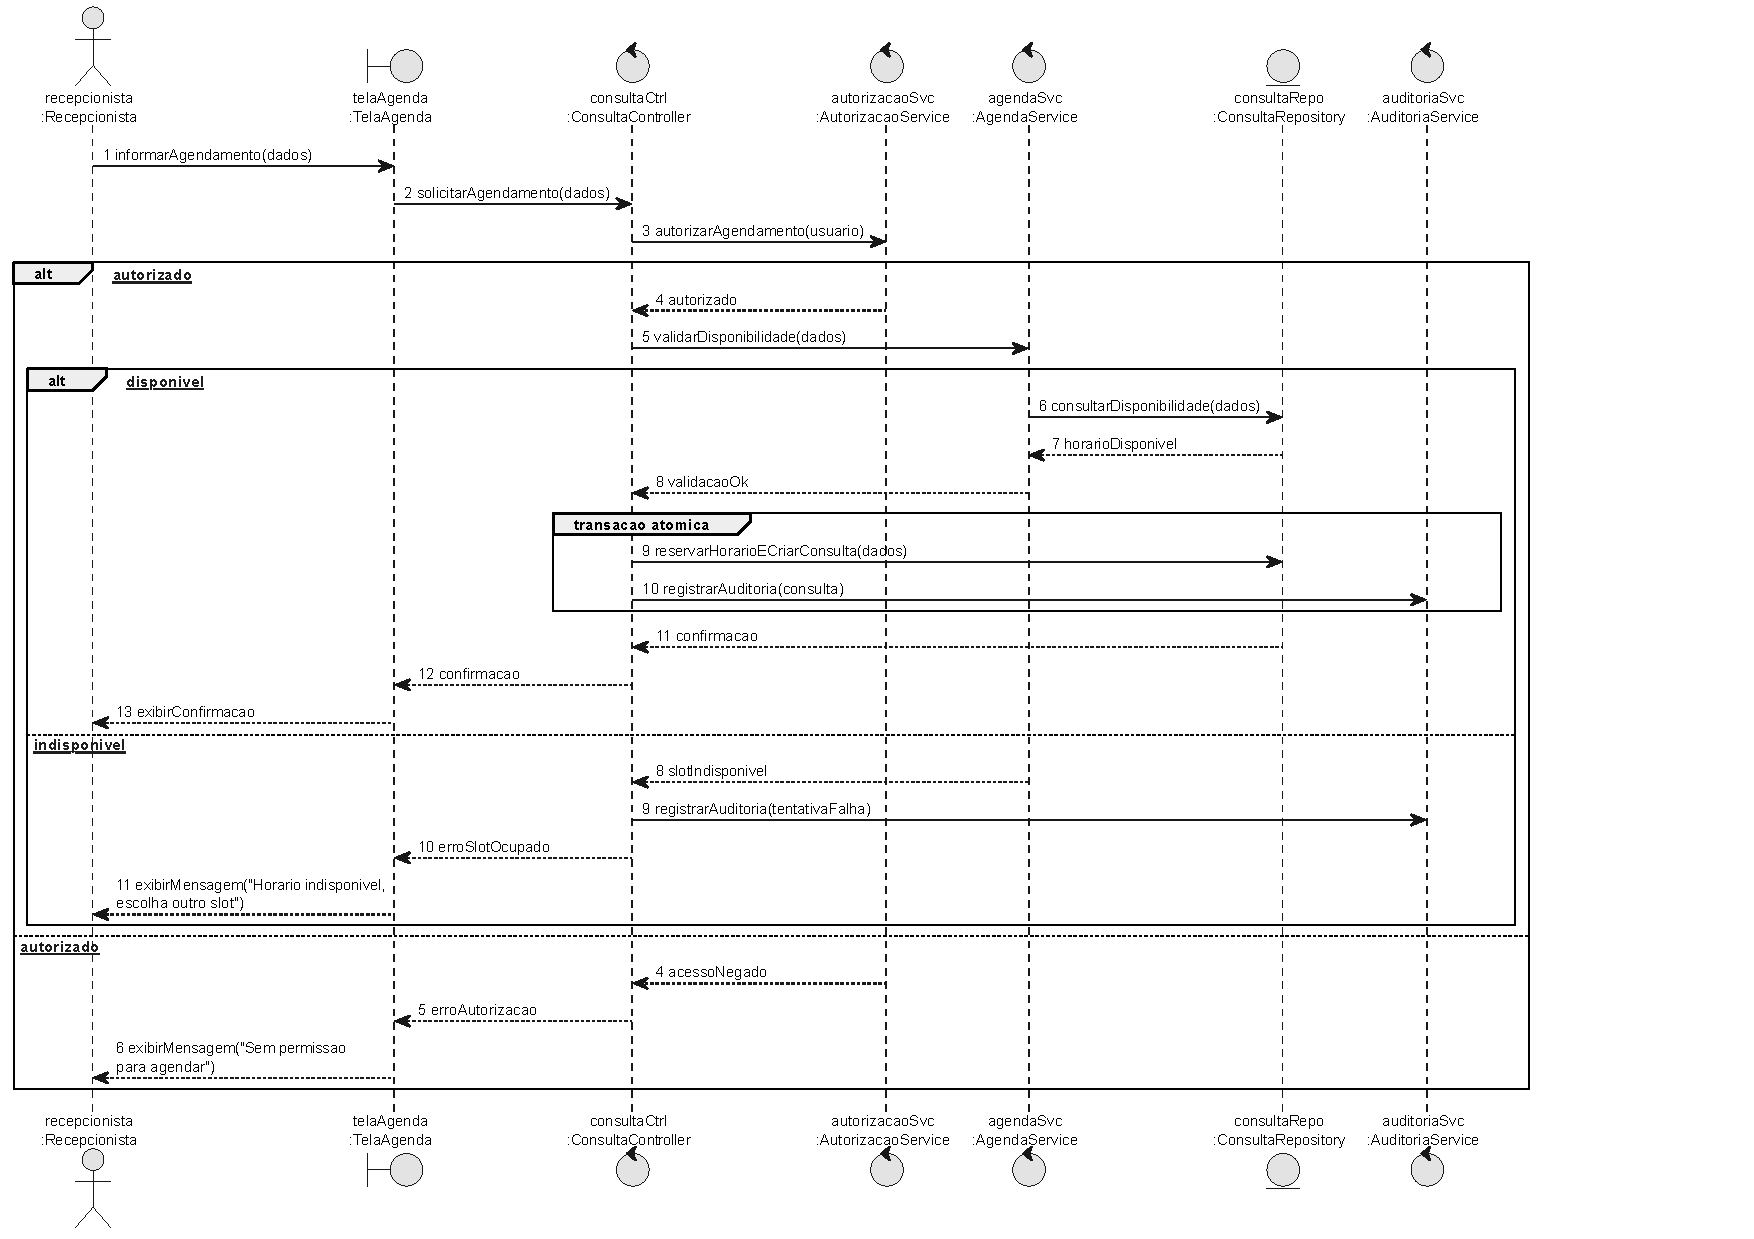
\includegraphics[
    width=0.95\linewidth,
    height=0.66\textheight,
    keepaspectratio
]{Imagens/arquitetura/M-V1-01-sequencia-agendamento}

\captionof{figure}{Modelo M-V1-01 -- Sequência de agendamento de consulta.}
\label{fig:m-v1-01-sequencia-agendamento}

\end{landscape}


% ---------------------------------------------------------
% Diagrama Modelo 2
% ---------------------------------------------------------
\begin{landscape}
\thispagestyle{plain}
\centering

{\scriptsize
\renewcommand{\arraystretch}{1.0}
\begin{tabular}{@{}lp{0.72\linewidth}@{}}
\textbf{View}           & V1 --- Visão de Cenários \\
\textbf{Model Kind}     & UML Sequence Diagram \\
\textbf{Concerns}       & C2 (Desempenho), C4 (Integridade Transacional), C5 (Auditoria), C8 (Interoperabilidade) \\
\textbf{Decisões}       & DA03 (RBAC), DA04 (Persistência Relacional Gerenciada), DA06 (Transações Atômicas), DA07 (Auditoria Centralizada) \\
\textbf{Participantes}  & \texttt{dispensacaoCtrl}: orquestra o fluxo; \texttt{autorizacaoSvc}: verifica permissão; \texttt{prescricaoSvc}: valida a prescrição; \texttt{estoqueService}: valida saldo e baixa estoque; \texttt{dispensacaoRepo}: persiste a dispensação; \texttt{auditoriaSvc}: registra o evento. \\
\end{tabular}
}

\vspace{0.3em}

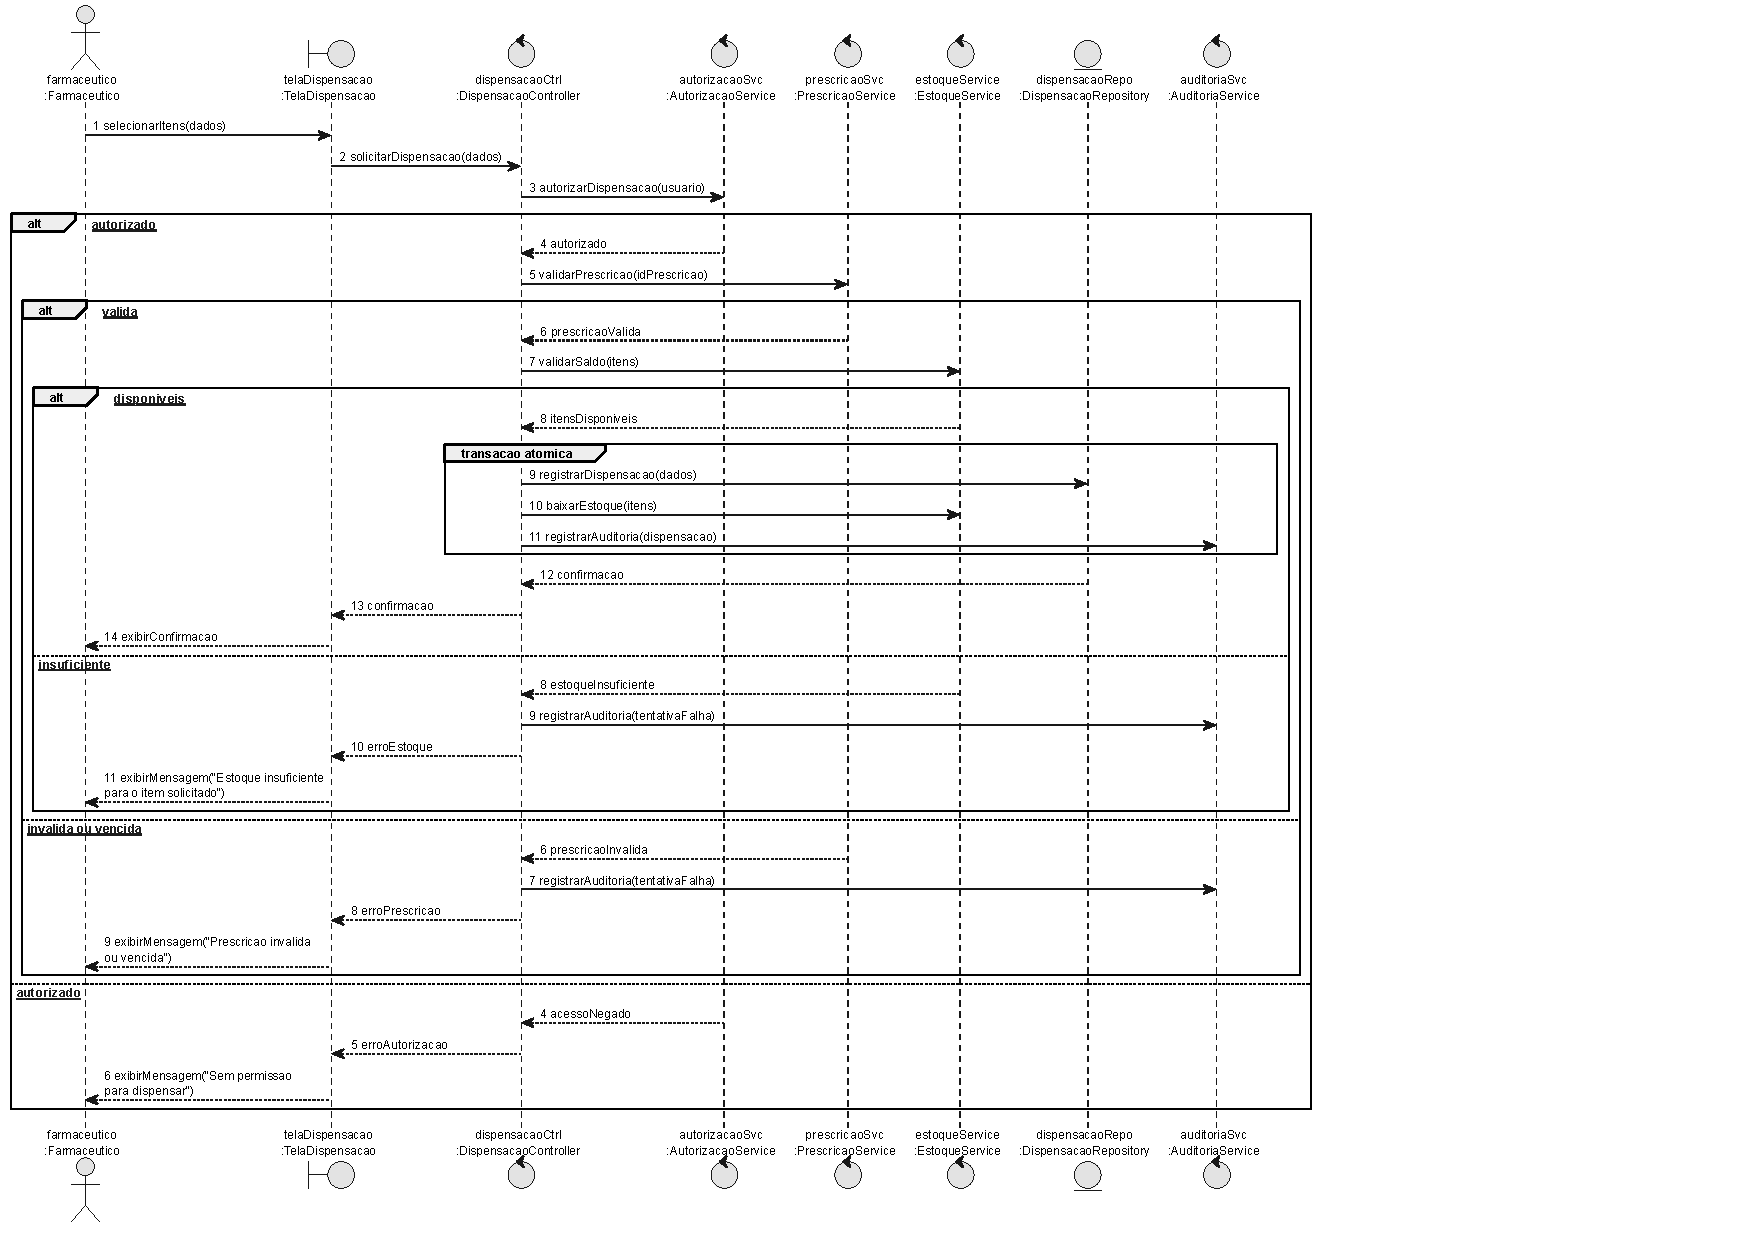
\includegraphics[
    width=0.95\linewidth,
    height=0.60\textheight,
    keepaspectratio
]{Imagens/arquitetura/M-V3-01-sequencia-dispensacao}

\captionof{figure}{Modelo M-V1-02 -- Sequência de dispensação transacional.}
\label{fig:m-v1-02-sequencia-dispensacao}

\end{landscape}


% ---------------------------------------------------------
% Diagrama Modelo 3
% ---------------------------------------------------------
\begin{landscape}
\thispagestyle{plain}
\centering

{\scriptsize
\renewcommand{\arraystretch}{1.0}
\begin{tabular}{@{}lp{0.72\linewidth}@{}}
\textbf{View}           & V1 --- Visão de Cenários \\
\textbf{Model Kind}     & UML Sequence Diagram \\
\textbf{Concerns}       & C1 (Controle de Acesso), C4 (Integridade Transacional), C5 (Auditoria), C9 (Usabilidade) \\
\textbf{Decisões}       & DA03 (RBAC), DA06 (Transações Atômicas), DA07 (Auditoria Centralizada) \\
\textbf{Participantes}  & \texttt{faturamentoCtrl}: orquestra o fluxo; \texttt{autorizacaoSvc}: verifica permissão; \texttt{consultaRepo}: recupera dados da consulta finalizada; \texttt{convenioSvc}: calcula cobertura; \texttt{contaMedicaRepo}: persiste conta e itens; \texttt{auditoriaSvc}: registra o evento. \\
\end{tabular}
}

\vspace{0.3em}

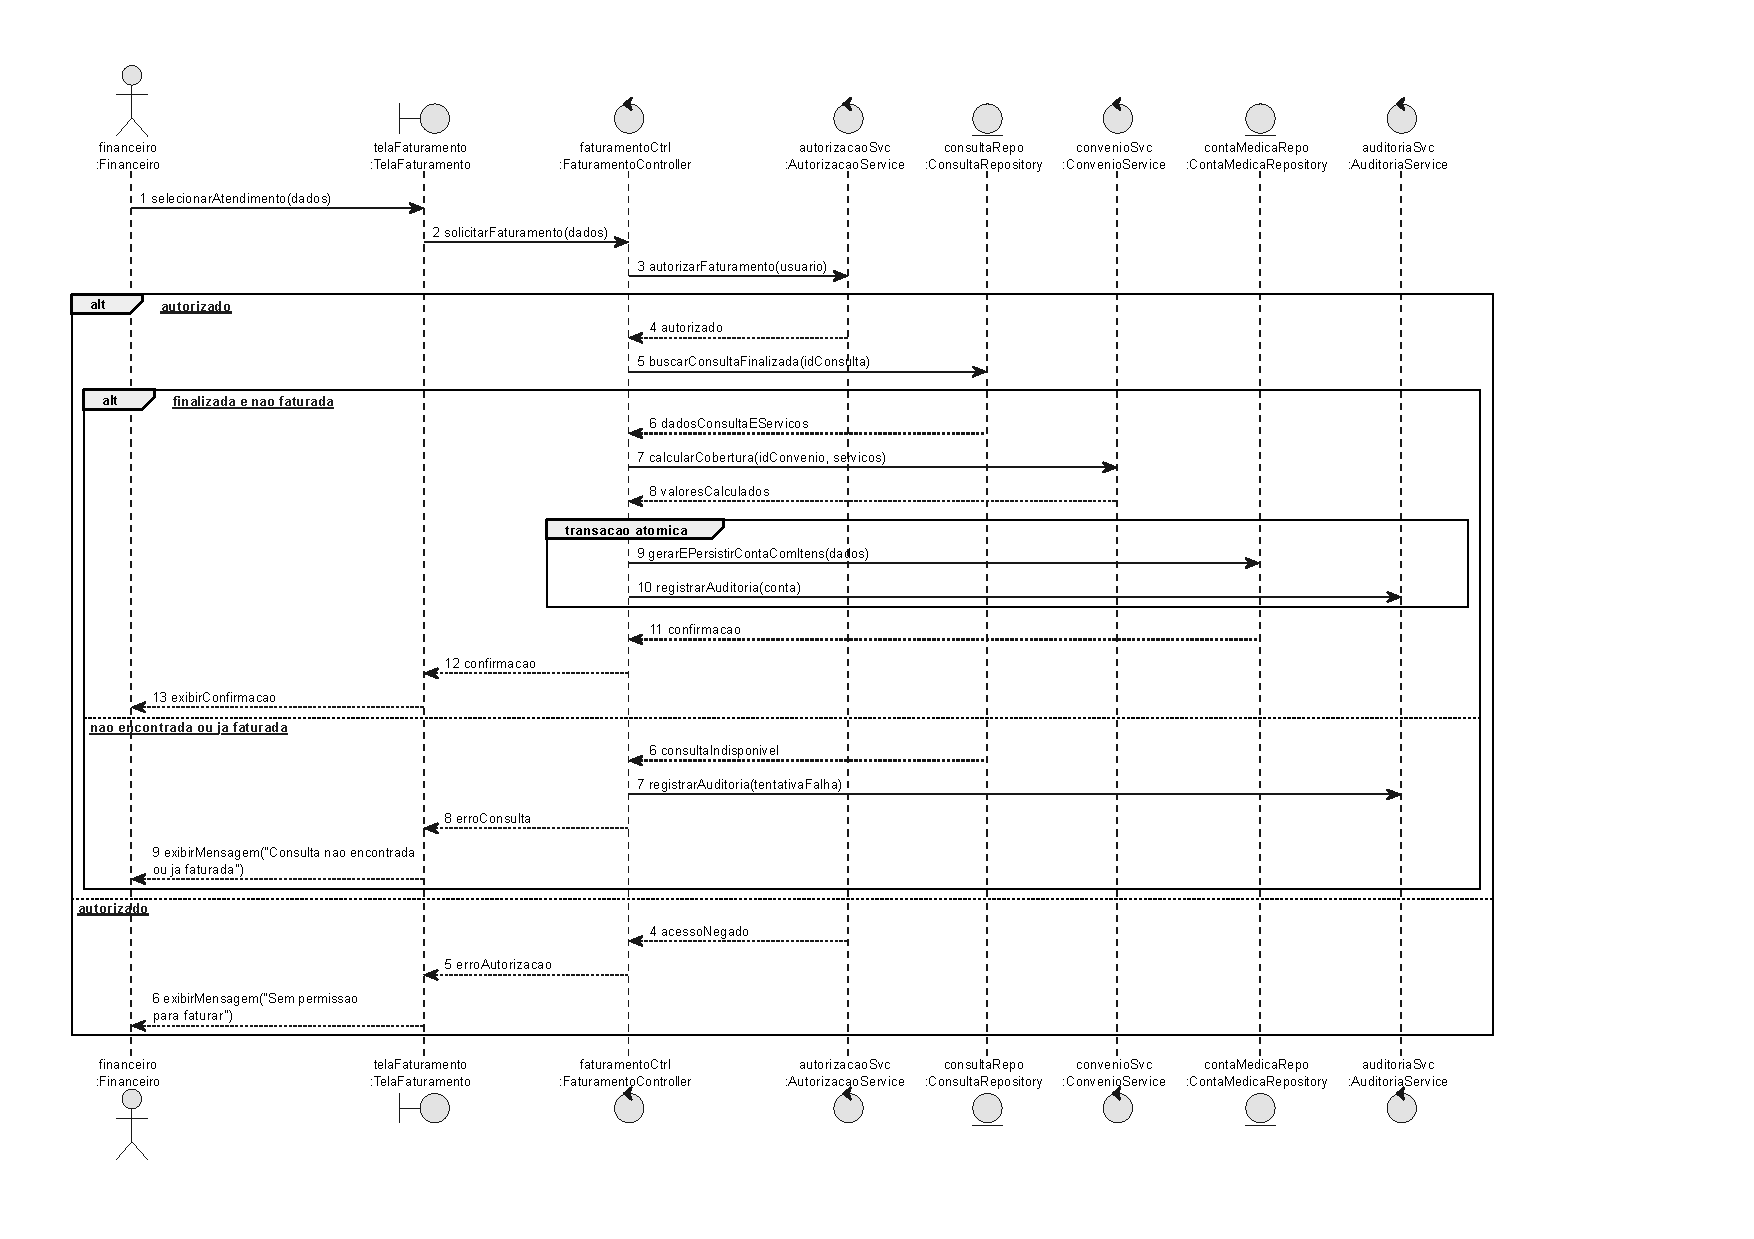
\includegraphics[
    width=0.92\linewidth,
    height=0.58\textheight,
    keepaspectratio,
    trim=0 80 0 0,
    clip
]{Imagens/arquitetura/M-V1-03-sequencia-faturamento}

\captionof{figure}{Modelo M-V1-03 -- Sequência de faturamento de atendimento.}
\label{fig:m-v1-03-sequencia-faturamento}

\end{landscape}


% ---------------------------------------------------------
% Diagrama Modelo 4 — Atendimento Clínico
% ---------------------------------------------------------
\begin{landscape}
\thispagestyle{plain}
\centering

{\scriptsize
\renewcommand{\arraystretch}{1.0}
\begin{tabular}{@{}lp{0.72\linewidth}@{}}
\textbf{View}           & V1 --- Visão de Cenários \\
\textbf{Model Kind}     & UML Sequence Diagram \\
\textbf{Concerns}       & C1 (Controle de Acesso), C4 (Integridade Transacional), C5 (Auditoria), C9 (Usabilidade) \\
\textbf{Decisões}       & DA01 (Arquitetura em Camadas), DA03 (RBAC), DA06 (Transações Atômicas), DA07 (Auditoria Centralizada) \\
\textbf{Participantes}  & \texttt{atendimentoCtrl}: orquestra o fluxo; \texttt{autorizacaoSvc}: verifica permissão; \texttt{consultaRepo}: recupera e atualiza status; \texttt{prontuarioRepo}: fornece histórico clínico; \texttt{atendimentoSvc}: aplica regras de negócio; \texttt{atendimentoRepo}: persiste atendimento; \texttt{auditoriaSvc}: registra eventos. \\
\end{tabular}
}

\vspace{0.3em}

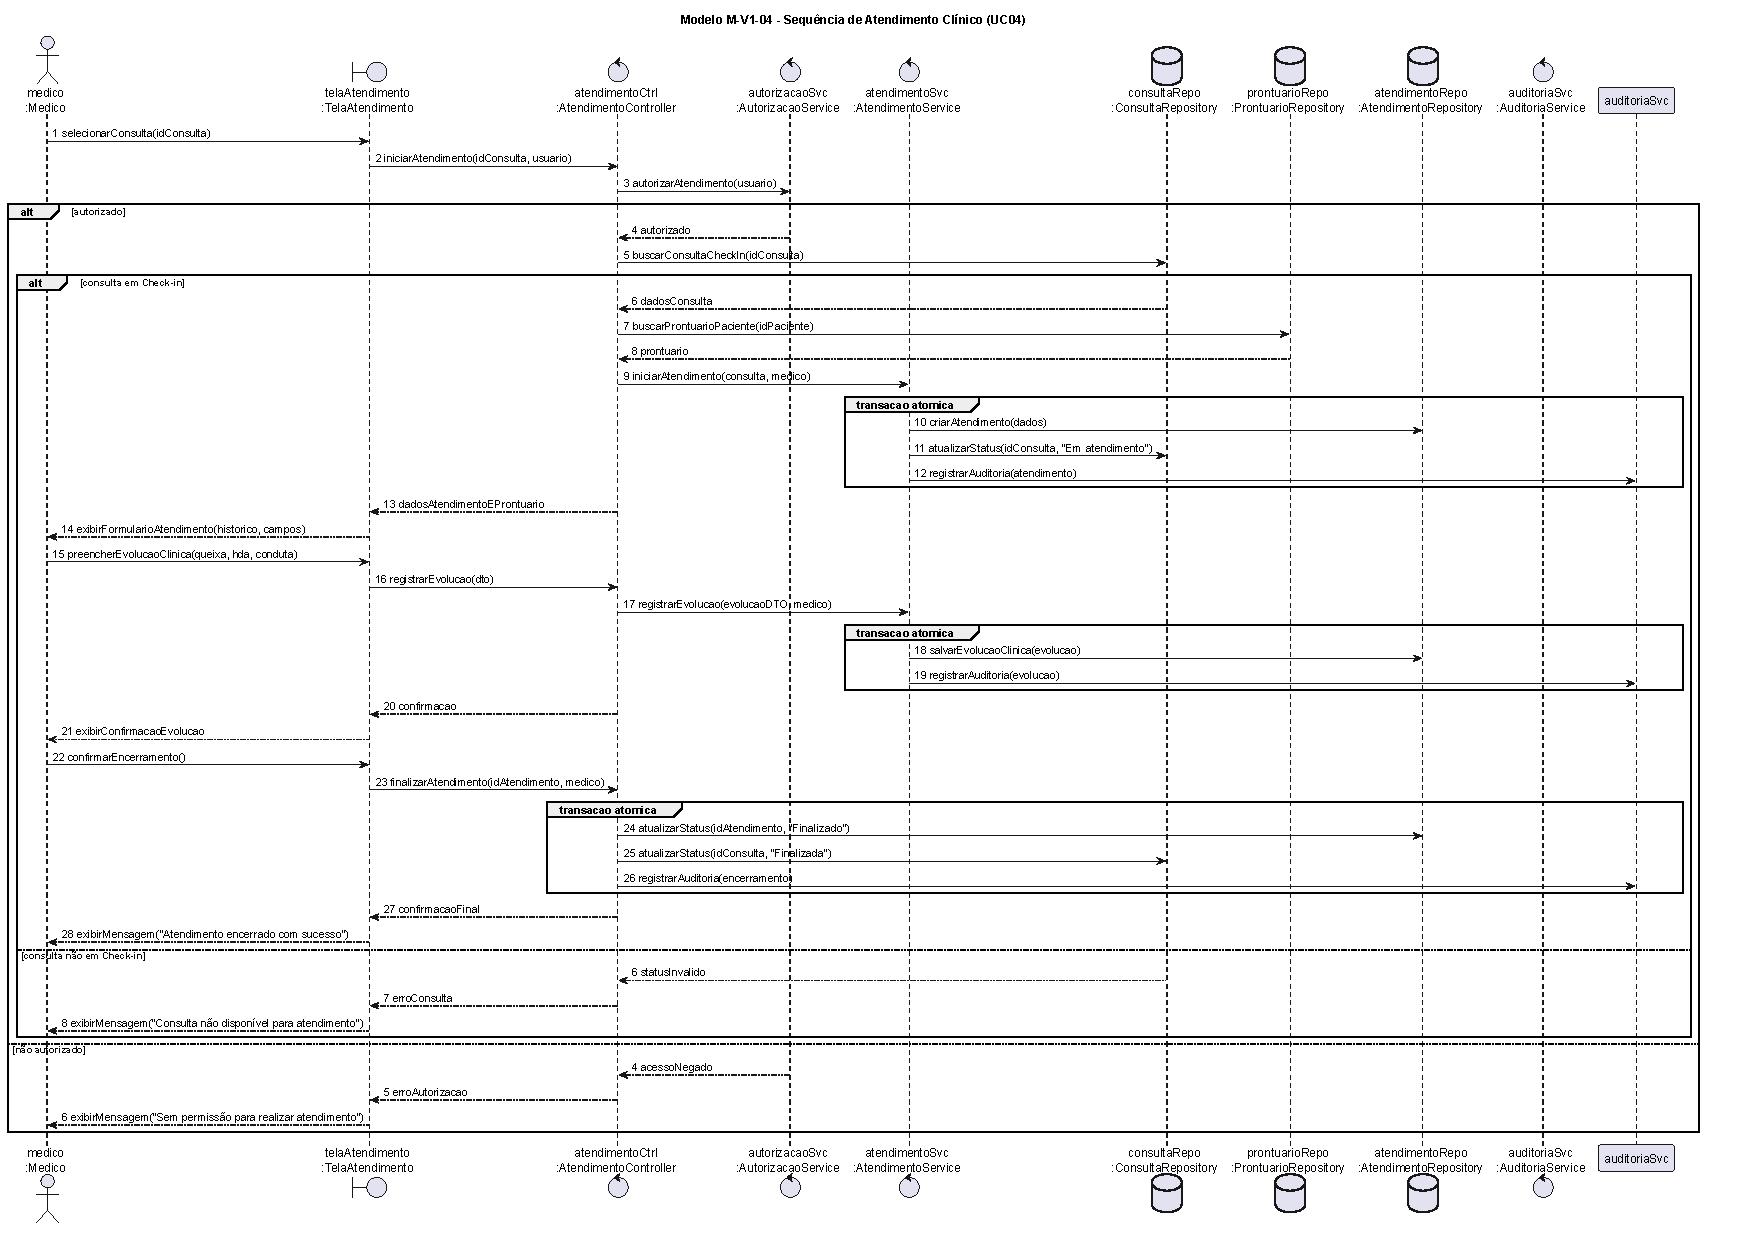
\includegraphics[
    width=0.95\linewidth,
    height=0.58\textheight,
    keepaspectratio
]{Imagens/arquitetura/M-V1-04_Sequencia_Atendimento_Clinico.pdf}

\captionof{figure}{Modelo M-V1-04 -- Sequência de atendimento clínico.}
\label{fig:m-v1-04-sequencia-atendimento}

\end{landscape}


% ---------------------------------------------------------
% Diagrama Modelo 5 — Autenticação RBAC
% ---------------------------------------------------------
\begin{landscape}
\thispagestyle{plain}
\centering

{\scriptsize
\renewcommand{\arraystretch}{1.0}
\begin{tabular}{@{}lp{0.72\linewidth}@{}}
\textbf{View}           & V1 --- Visão de Cenários \\
\textbf{Model Kind}     & UML Sequence Diagram \\
\textbf{Concerns}       & C1 (Controle de Acesso), C5 (Auditoria), C6 (Conformidade com LGPD) \\
\textbf{Decisões}       & DA03 (RBAC), DA07 (Auditoria Centralizada) \\
\textbf{Participantes}  & \texttt{authCtrl}: recebe credenciais e orquestra autenticação; \texttt{authSvc}: valida senha, MFA e gera token; \texttt{usuarioRepo}: recupera dados do usuário; \texttt{rbacSvc}: carrega perfis e permissões; \texttt{permissaoRepo}: fornece permissões; \texttt{auditoriaSvc}: registra tentativas e resultados. \\
\end{tabular}
}

\vspace{0.3em}

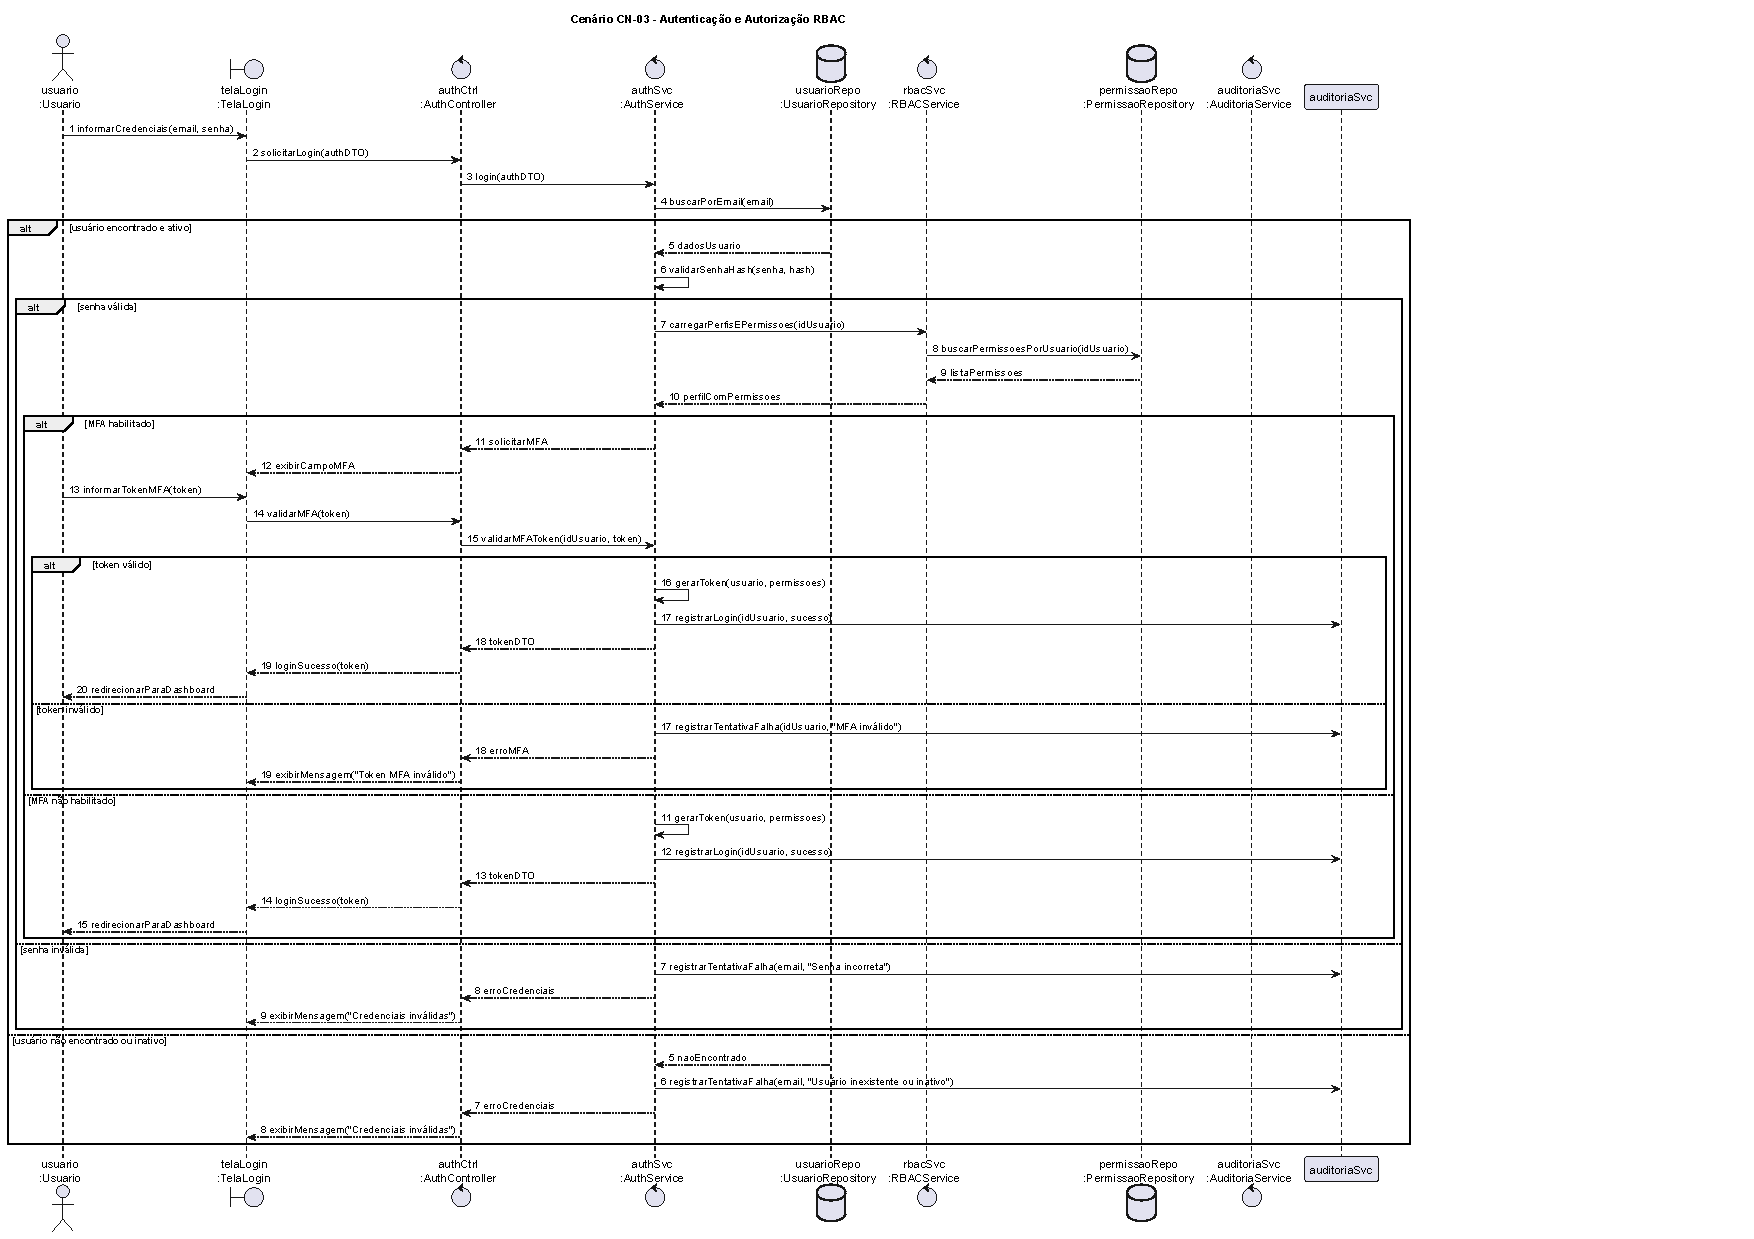
\includegraphics[
    width=0.95\linewidth,
    height=0.58\textheight,
    keepaspectratio
]{Imagens/arquitetura/M-V1-CN03_Sequencia_Autenticacao_RBAC.pdf}

\captionof{figure}{Modelo M-V1-05 -- Sequência de autenticação e autorização RBAC (CN-03).}
\label{fig:m-v1-05-sequencia-autenticacao-rbac}

\end{landscape}

% ---------------------------------------------------------
% Diagramas de Estados
% ---------------------------------------------------------
\section{Diagramas de Estados}

Os diagramas de estados (DTE) mostram o ciclo de vida de um objeto específico, ou seja, por quais situações (estados) ele passa desde a sua criação até a sua destruição/finalização.

\subsection{Ciclo de Vida de uma Consulta}

O diagrama a seguir modela o ciclo de vida completo da entidade \texttt{Consulta} no SGC, mapeando os oito estados possíveis definidos no esquema relacional e os eventos de negócio que disparam cada transição. A partir do estado inicial \textit{Agendada}, criado quando a recepcionista registra uma nova consulta, o fluxo avança por \textit{Confirmada}, \textit{Check-in} e \textit{Em atendimento} até o estado \textit{Finalizada}, quando o médico encerra e salva o prontuário. O estado \textit{Faturada}, atingido após o processamento financeiro, representa o encerramento natural do ciclo. O estado \textit{Remarcada} é transitório: a consulta retorna a \textit{Agendada} com novo horário definido. O estado \textit{Cancelada} pode ser atingido a partir de \textit{Agendada} ou \textit{Confirmada} e, juntamente com \textit{Faturada}, conduz ao estado final do diagrama.

\begin{figure}[htbp]
\centering

\begin{center}
\small
\renewcommand{\arraystretch}{1.3}
\begin{tabular}{ll}
\textbf{View}        & V1 --- Visão de Cenários \\
\textbf{Model Kind}  & UML State Diagram \\
\textbf{Concerns}    & C4 (Integridade Transacional), C7 (Modularidade) \\
\textbf{Decisões}    & DA06 (Transações Atômicas) \\
\end{tabular}
\end{center}

\vspace{1em}

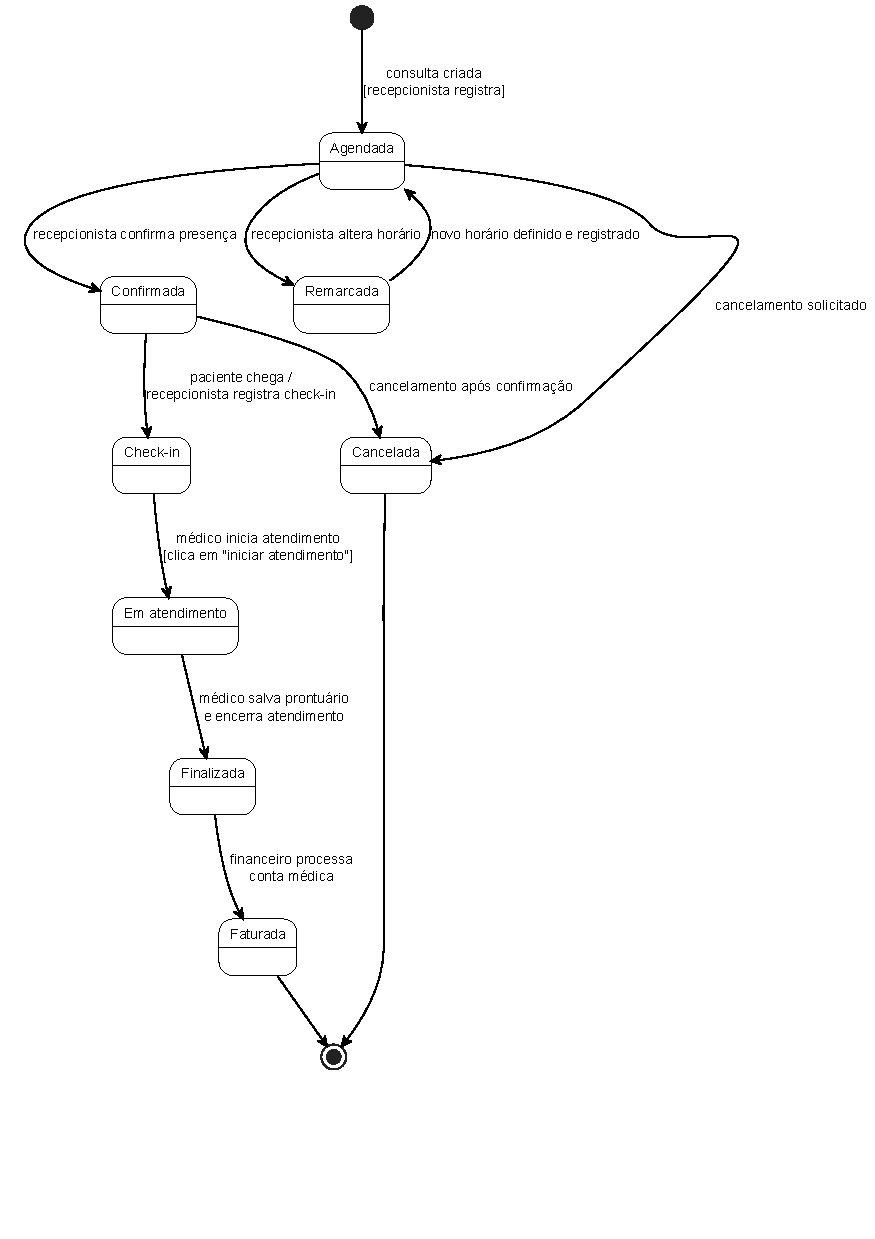
\includegraphics[
    width=0.85\linewidth,
    height=0.95\textheight,
    keepaspectratio
]{Imagens/arquitetura/DTE-ciclo-vida-consulta}

\caption{Ciclo de vida da entidade Consulta.}
\label{fig:dte-ciclo-vida-consulta}

\end{figure}

% ---------------------------------------------------------
% DTE — Prescrição
% ---------------------------------------------------------
\subsection{Ciclo de Vida de uma Prescrição}

O diagrama a seguir modela o ciclo de vida da entidade \texttt{Prescricao} no SGC. A partir do estado \textit{Emitida}, gerado quando o médico confirma a prescrição ao término ou durante o atendimento, o fluxo pode avançar para \textit{Dispensada Parcialmente}, caso a farmácia realize a entrega de apenas parte dos itens prescritos, ou diretamente para \textit{Dispensada}, quando todos os itens são entregues de uma vez. Cancelamentos são permitidos enquanto nenhum ou apenas parte dos itens tiver sido dispensado. O estado \textit{Dispensada} e o estado \textit{Cancelada} conduzem ao estado final do ciclo.

\begin{figure}[htbp]
\centering

\begin{center}
\small
\renewcommand{\arraystretch}{1.3}
\begin{tabular}{ll}
\textbf{View}        & V1 --- Visão de Cenários \\
\textbf{Model Kind}  & UML State Diagram \\
\textbf{Concerns}    & C4 (Integridade Transacional), C5 (Auditoria), C10 (Persistência e Consistência) \\
\textbf{Decisões}    & DA06 (Transações Atômicas), DA07 (Auditoria Centralizada) \\
\end{tabular}
\end{center}

\vspace{1em}

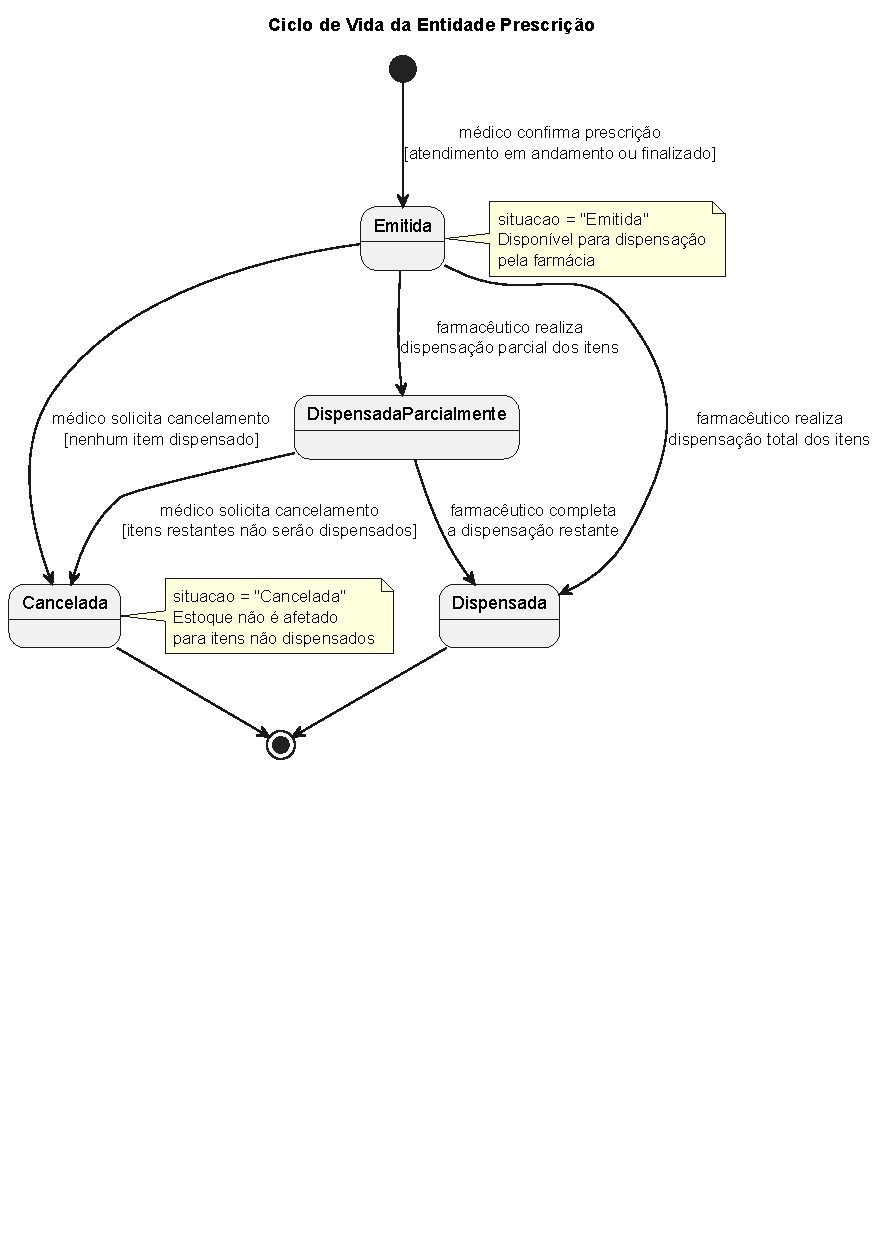
\includegraphics[
    width=0.75\linewidth,
    height=0.95\textheight,
    keepaspectratio
]{Imagens/arquitetura/DTE_Prescricao.pdf}

\caption{Ciclo de vida da entidade Prescrição.}
\label{fig:dte-ciclo-vida-prescricao}

\end{figure}


% ---------------------------------------------------------
% DTE — ContaMedica
% ---------------------------------------------------------
\subsection{Ciclo de Vida de uma Conta Médica}

O diagrama a seguir modela o ciclo de vida da entidade \texttt{ContaMedica} no SGC. A partir do estado \textit{Pendente}, gerado automaticamente após o processamento financeiro de uma consulta finalizada, a conta pode ser encaminhada para \textit{Em Análise} quando o convênio solicita revisão dos valores. Após a análise, os valores podem ser recalculados e a conta retorna a \textit{Pendente}, ou o convênio aprova e efetua o pagamento, conduzindo ao estado \textit{Pago}. Cancelamentos são permitidos a partir dos estados \textit{Pendente} e \textit{Em Análise}. Os estados \textit{Pago} e \textit{Cancelado} conduzem ao estado final do ciclo.

\begin{figure}[htbp]
\centering

\begin{center}
\small
\renewcommand{\arraystretch}{1.3}
\begin{tabular}{ll}
\textbf{View}        & V1 --- Visão de Cenários \\
\textbf{Model Kind}  & UML State Diagram \\
\textbf{Concerns}    & C4 (Integridade Transacional), C5 (Auditoria), C10 (Persistência e Consistência) \\
\textbf{Decisões}    & DA06 (Transações Atômicas), DA07 (Auditoria Centralizada) \\
\end{tabular}
\end{center}

\vspace{1em}

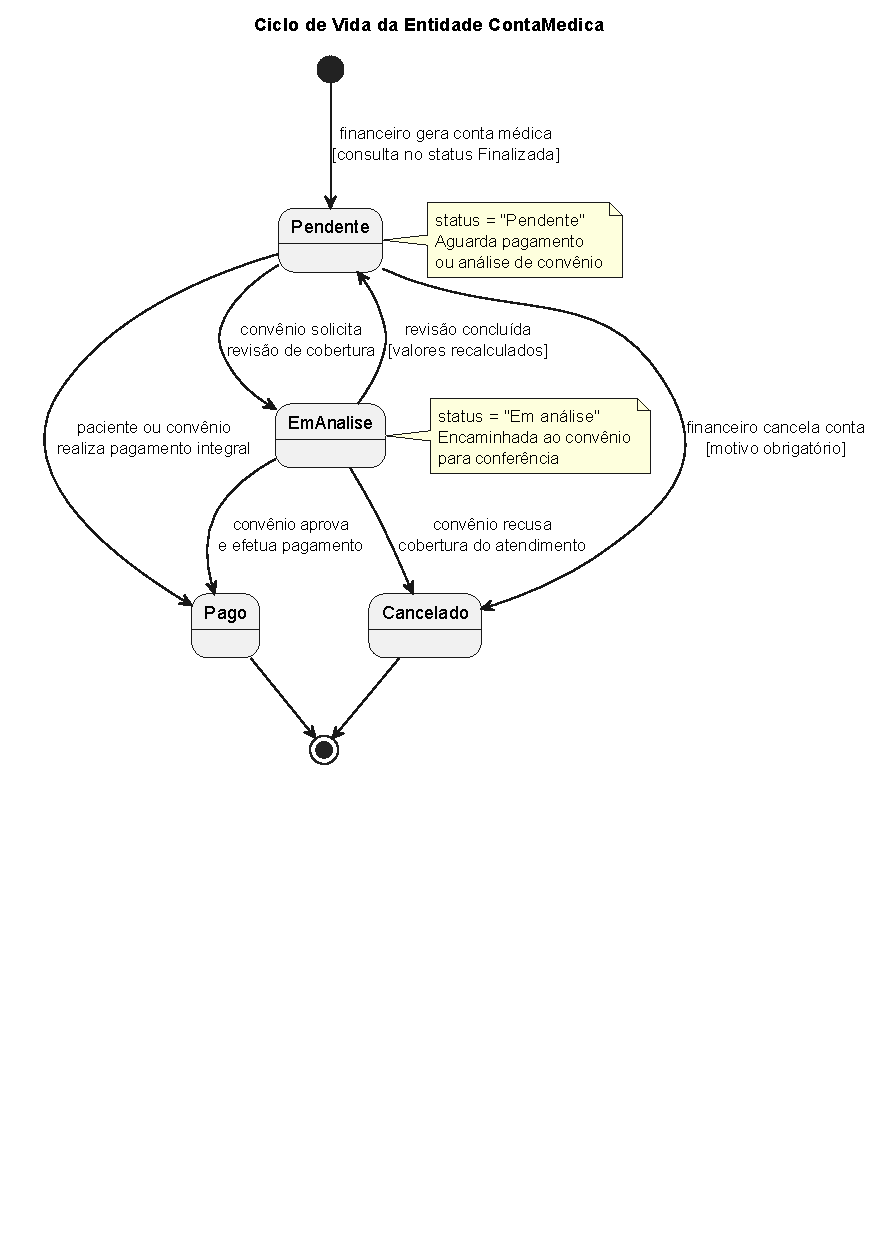
\includegraphics[
    width=0.75\linewidth,
    height=0.95\textheight,
    keepaspectratio
]{Imagens/arquitetura/DTE_ContaMedica.pdf}

\caption{Ciclo de vida da entidade ContaMedica.}
\label{fig:dte-ciclo-vida-conta-medica}

\end{figure}

% ---------------------------------------------------------
% Diagrama de Atividades
% ---------------------------------------------------------
\section{Diagrama de Atividades}

O diagrama de atividades é um fluxograma estendido que permite representar ações concorrentes, regras lógicas, sincronização e a divisão de tarefas por atores utilizando raias (\textit{swimlanes}).

\subsection{Processo de Triagem e Atendimento Clínico}

O diagrama a seguir descreve o processo colaborativo de triagem e atendimento clínico, baseando-se nos casos de uso UC02 (Gerenciar Agenda de Consultas), UC04 (Realizar Atendimento Clínico) e UC05 (Emitir Prescrição Médica). O fluxo é organizado em três raias (\textit{swimlanes}): \textbf{Recepcionista}, responsável pelo acolhimento do paciente e pelo registro do check-in; \textbf{Sistema (SGC)}, que valida a presença, atualiza o status da consulta e disponibiliza o prontuário na fila médica; e \textbf{Médico}, que conduz o atendimento clínico, preenche a evolução e decide sobre a necessidade de prescrição ou exames. Uma bifurcação lógica determina se a consulta gera ou não uma prescrição vinculada, após o que o médico confirma o encerramento e o sistema atualiza o status da consulta para \textit{Finalizada}.


\begin{landscape}
\thispagestyle{plain}

\begin{center}
\begin{minipage}{0.98\linewidth}

\begin{center}
\small
\renewcommand{\arraystretch}{1.2}
\begin{tabular}{lp{0.75\linewidth}}
\textbf{View}        & V1 --- Visão de Cenários \\
\textbf{Model Kind}  & UML Activity Diagram \\
\textbf{Concerns}    & C2 (Desempenho), C4 (Integridade Transacional), C9 (Usabilidade) \\
\textbf{Decisões}    & DA01 (Arquitetura em Camadas), DA06 (Transações Atômicas) \\
\end{tabular}
\end{center}

\vspace{0.6em}

\centering
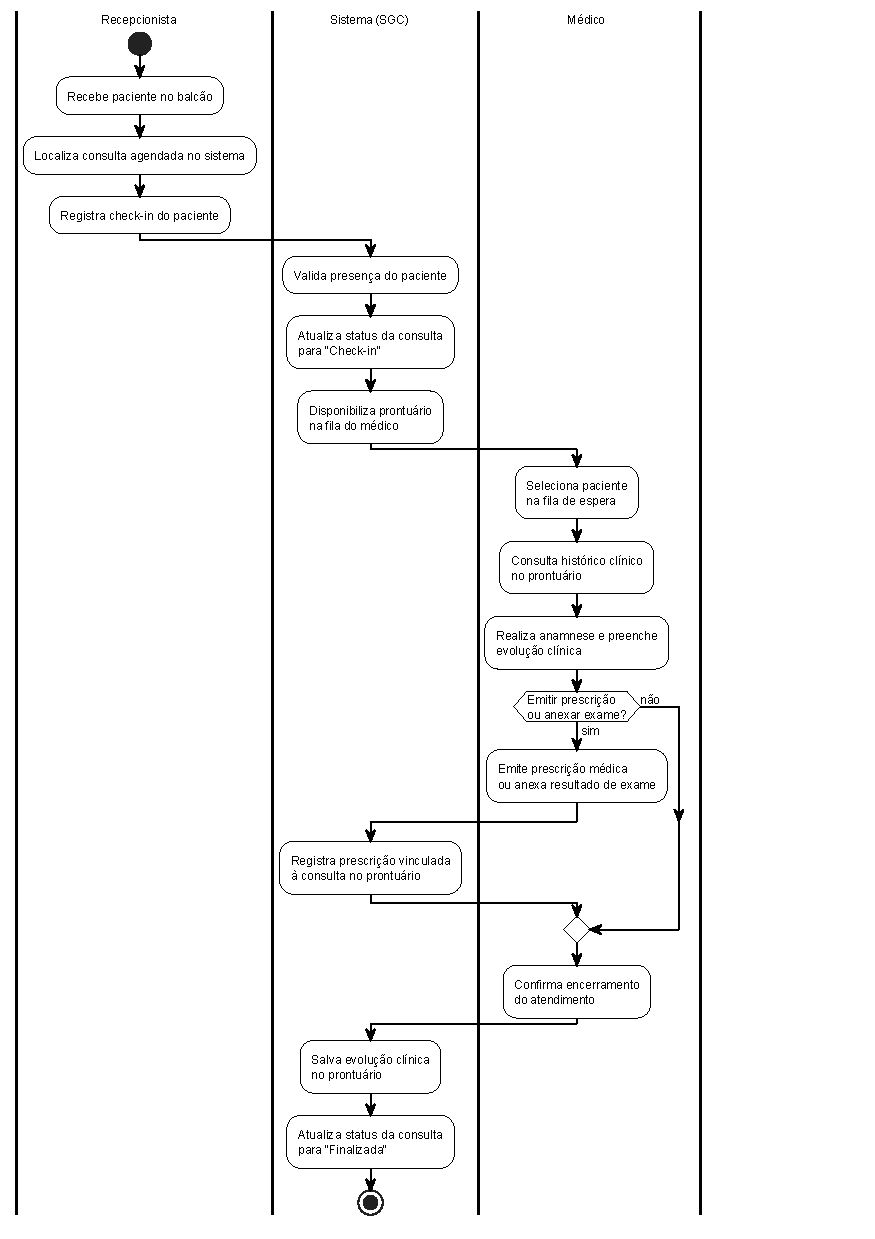
\includegraphics[
    width=0.98\linewidth,
    height=0.82\textheight,
    keepaspectratio
]{Imagens/arquitetura/DA-triagem-atendimento}

\captionof{figure}{Diagrama de atividades -- Processo de triagem e atendimento clínico.}
\label{fig:da-triagem-atendimento}

\end{minipage}
\end{center}

\end{landscape}

\chapter{Arquitetura do Software}

%% ─────────────────────────────────────────────
\section{Abordagem de Descrição Arquitetural}

A descrição arquitetural do Sistema de Gestão de Clínica (SGC) segue a norma \textbf{ISO/IEC/IEEE 42010:2022}, que define um framework conceitual para a expressão, comunicação e revisão de arquiteturas de sistemas de software. Segundo essa norma, a descrição arquitetural deve registrar as decisões de design que satisfazem os concerns das partes interessadas, organizando-as em \textit{viewpoints} e \textit{views} com seus respectivos modelos.

Adicionalmente, a estrutura da descrição segue o modelo de maturidade \textbf{ArchCaMo} (\textit{Architecture Completeness Model}), que permite avaliar o grau de completude e rastreabilidade dos artefatos arquiteturais. Cada seção deste capítulo corresponde a elementos do ArchCaMo, garantindo aderência ao nível de completude esperado para projetos de software clínico.

A elaboração das \textit{views} e modelos considera também a norma \textbf{ISO/IEC/IEEE 42020:2019}, especialmente a atividade de elaboração arquitetural, que orienta como arquiteturas devem ser criadas, analisadas e avaliadas de forma sistemática no contexto do sistema de interesse.

%% ─────────────────────────────────────────────
\section{Sistema de Interesse, Ambiente e Escopo Arquitetural}

O \textbf{sistema de interesse} é o SGC --- um sistema de software para gestão integral de clínicas de saúde, compreendendo os módulos de agendamento, prontuário eletrônico, farmácia clínica, faturamento, controle de acesso e gestão de recursos físicos.

O \textbf{ambiente} é composto por: clínicas de pequeno e médio porte, usuários internos (recepcionistas, médicos, farmacêuticos, administradores), operadores de convênios e plataforma em nuvem com acesso via navegador web.

O \textbf{escopo arquitetural} abrange:
\begin{itemize}
    \item A estrutura interna do sistema e seus componentes de software;
    \item As interações entre os módulos e a camada de persistência;
    \item Os mecanismos de segurança, auditoria e controle de acesso;
    \item A estratégia de implantação em ambiente de nuvem.
\end{itemize}

Estão \textbf{fora do escopo}: integrações com sistemas de saúde externos (e.g., TISS, HL7), equipamentos médicos, aplicativos móveis para pacientes e módulos de telemedicina.

%% ─────────────────────────────────────────────
\section{Stakeholders e Concerns Arquiteturais}
 
\subsection{Stakeholders Arquiteturais}
 
Os stakeholders foram decompostos em perfis atômicos, cada um com responsabilidades
e interesses distintos sobre a arquitetura. A \autoref{tab:stakeholders-arquitetura}
apresenta os onze perfis identificados.
 
\begin{table}[H]
\caption{Stakeholders arquiteturais e concerns associados.}
\label{tab:stakeholders-arquitetura}
\centering
\small
\begin{tabularx}{\textwidth}{|l|l|X|l|}
\hline
\textbf{ID} & \textbf{Stakeholder} & \textbf{Responsabilidade principal} & \textbf{Concerns} \\
\hline
S1  & Desenvolvedor front-end     & Implementa a interface React e consome a API REST & C7, C8, C9, C11 \\
\hline
S2  & Desenvolvedor back-end      & Implementa regras de negócio, endpoints e transações & C4, C7, C8, C11 \\
\hline
S3  & Administrador de sistemas   & Configura usuários, perfis e audita operações sensíveis & C1, C5, C6 \\
\hline
S4  & Médico / Clínico            & Registra atendimentos, evolução clínica e prescrições & C2, C4, C9 \\
\hline
S5  & Recepcionista               & Gerencia agenda de consultas e cadastros de pacientes & C2, C4, C9 \\
\hline
S6  & Farmacêutico                & Realiza dispensações e controla estoque de medicamentos & C4, C5, C10 \\
\hline
S7  & Financeiro                  & Gera cobranças, confere convênios e emite comprovantes & C4, C9, C10 \\
\hline
S8  & DevOps     & Mantém infraestrutura, monitora serviços e executa deploys & C3, C10, C12 \\
\hline
S9  & Responsável pela conformidade (DPO) & Verifica aderência à LGPD e conduz auditorias & C5, C6, C1 \\
\hline
S10 & Paciente                    & Recebe confirmações de consulta e comprovantes & C2, C9 \\
\hline
S11 & Gestor da clínica           & Acompanha relatórios financeiros e operacionais & C5, C9, C12 \\
\hline
\end{tabularx}
\end{table}
 
\subsection{Concerns Arquiteturais}
 
Os \textit{concerns} representam os interesses, objetivos e restrições que a
arquitetura deve satisfazer. Para cada concern, descreve-se o interesse geral e,
em seguida, como cada stakeholder o interpreta de forma particular.
 
\begin{longtable}{|l|l|p{9.5cm}|}
\caption{Concerns arquiteturais do SGC com perspectiva por stakeholder.}
\label{tab:concerns-arquitetura} \\
\hline
\textbf{ID} & \textbf{Concern} & \textbf{Descrição geral e perspectiva por stakeholder} \\
\hline
\endfirsthead
\hline
\textbf{ID} & \textbf{Concern} & \textbf{Descrição geral e perspectiva por stakeholder} \\
\hline
\endhead
\hline
\endfoot
 
C1 & Controle de acesso e segurança &
Somente usuários autorizados executam operações sensíveis; autenticação robusta e RBAC granular.
\newline\textbf{S3 (Admin. sistemas):} precisa criar, inativar e auditar contas sem expor o sistema a escalada de privilégios.
\newline\textbf{S9 (DPO):} exige que nenhum dado de paciente seja acessível a perfis não autorizados, com rastreio de cada acesso. \\
\hline
C2 & Desempenho e responsividade &
Tempos de resposta aceitáveis nas operações cotidianas.
\newline\textbf{S4 (Médico):} espera que a abertura do prontuário e o registro de evolução respondam em menos de dois segundos durante o atendimento.
\newline\textbf{S5 (Recepcionista):} precisa que o calendário de agendamentos carregue sem atraso perceptível ao receber pacientes em fila.
\newline\textbf{S10 (Paciente):} aguarda confirmação de consulta imediata no balcão ou por canal digital. \\
\hline
C3 & Disponibilidade e continuidade &
Sistema operacional mesmo em falhas parciais; recuperação e backups automáticos.
\newline\textbf{S8 (DevOps):} requer que falhas em um contêiner não derrubem o sistema inteiro e que backups sejam verificáveis. \\
\hline
C4 & Integridade transacional &
Atomicidade nas operações críticas: nenhuma escrita parcial deve ser persistida.
\newline\textbf{S2 (Dev. back-end):} implementa transações ACID nos serviços de agendamento, dispensação e faturamento.
\newline\textbf{S4 (Médico):} o prontuário deve refletir exatamente o que foi salvo; uma falha não pode corromper o registro clínico.
\newline\textbf{S5 (Recepcionista):} dois recepcionistas não podem confirmar o mesmo slot simultaneamente.
\newline\textbf{S6 (Farmacêutico):} a baixa de estoque e o registro de dispensação devem ocorrer atomicamente.
\newline\textbf{S7 (Financeiro):} a cobrança e os itens de conta devem ser gerados ou revertidos juntos. \\
\hline
C5 & Rastreabilidade e auditoria &
Registro completo e imutável de operações para auditoria, conformidade e investigação.
\newline\textbf{S3 (Admin. sistemas):} precisa consultar quem alterou permissões ou inativou cadastros.
\newline\textbf{S6 (Farmacêutico):} toda dispensação deve ter rastro de lote, quantidade e responsável.
\newline\textbf{S9 (DPO):} os logs de acesso a dados pessoais devem ser preservados pelo período legal.
\newline\textbf{S11 (Gestor):} relatórios de operações realizadas por período devem ser geráveis a qualquer momento. \\
\hline
C6 & Conformidade com LGPD &
Proteção de dados pessoais e sensíveis de pacientes conforme a Lei 13.709/2018.
\newline\textbf{S3 (Admin. sistemas):} garante que dados só sejam acessados por usuários com finalidade justificada.
\newline\textbf{S9 (DPO):} exige criptografia em repouso para arquivos clínicos, anonimização em relatórios e política de retenção de dados. \\
\hline
C7 & Modularidade e manutenibilidade &
Módulos coesos e de baixo acoplamento, facilitando evoluções e manutenções independentes.
\newline\textbf{S1 (Dev. front-end):} quer consumir contratos de API estáveis sem depender de detalhes do back-end.
\newline\textbf{S2 (Dev. back-end):} quer alterar a lógica de farmácia sem risco de quebrar o módulo de agendamento. \\
\hline
C8 & Interoperabilidade entre módulos &
Comunicação padronizada entre módulos internos via interfaces bem definidas.
\newline\textbf{S1 (Dev. front-end):} consome a API via contrato OpenAPI; mudanças de implementação não devem exigir retrabalho no cliente.
\newline\textbf{S2 (Dev. back-end):} os módulos de domínio se comunicam por interfaces de serviço; nenhum módulo acessa diretamente o repositório de outro. \\
\hline
C9 & Experiência e usabilidade &
Interface intuitiva e responsiva, adequada ao fluxo de trabalho clínico.
\newline\textbf{S4 (Médico):} o formulário de evolução deve ser rápido de preencher sem alternar entre múltiplas telas.
\newline\textbf{S5 (Recepcionista):} o calendário deve permitir criar e remarcar consultas com poucos cliques.
\newline\textbf{S7 (Financeiro):} as telas de cobrança devem exibir os valores calculados antes de confirmar.
\newline\textbf{S10 (Paciente):} confirmações e comprovantes devem ser legíveis e imediatos.
\newline\textbf{S11 (Gestor):} painéis de relatório devem ser compreensíveis sem treinamento técnico. \\
\hline
C10 & Persistência e consistência &
Durabilidade dos dados e consistência entre banco relacional e storage de arquivos clínicos.
\newline\textbf{S6 (Farmacêutico):} os saldos de estoque devem refletir cada dispensação em tempo real.
\newline\textbf{S7 (Financeiro):} os valores faturados não podem divergir do que está registrado nas cobranças.
\newline\textbf{S8 (DevOps):} backups do banco e do storage devem ser sincronizados e restauráveis de forma consistente. \\
\hline
C11 & Testabilidade e qualidade &
Código estruturado para testes unitários, de integração e regressão automatizados.
\newline\textbf{S1 (Dev. front-end):} componentes React devem ser testáveis isoladamente com dados mockados.
\newline\textbf{S2 (Dev. back-end):} serviços de domínio devem ser injetáveis e testáveis sem depender do banco real. \\
\hline
C12 & Operação e implantação &
Implantação automatizada, monitoramento contínuo e rollback seguro em nuvem.
\newline\textbf{S8 (DevOps):} o pipeline CI/CD deve implantar novas versões sem downtime e permitir rollback em um comando.
\newline\textbf{S11 (Gestor):} precisa saber o status operacional do sistema sem depender da equipe técnica para obter essa informação. \\
\hline
 
\end{longtable}
 
\subsection{Matriz Concern--Stakeholder}
 
A \autoref{tab:matriz-concern-stakeholder} relaciona cada concern com os stakeholders
afetados, utilizando \textbf{P} (primário) e \textbf{S} (secundário).
 
\begin{table}[H]
\caption{Matriz Concern--Stakeholder.}
\label{tab:matriz-concern-stakeholder}
\centering
\footnotesize
\setlength{\tabcolsep}{4pt}
\begin{tabularx}{\textwidth}{|X|*{11}{>{\centering\arraybackslash}p{0.85cm}|}}
\hline
\textbf{Concern}
  & \textbf{S1} & \textbf{S2} & \textbf{S3} & \textbf{S4}
  & \textbf{S5} & \textbf{S6} & \textbf{S7} & \textbf{S8}
  & \textbf{S9} & \textbf{S10} & \textbf{S11} \\
\hline
C1 -- Acesso/Segurança     & -- & -- & P  & S  & S  & S  & --  & S  & P  & --  & -- \\
C2 -- Desempenho           & S  & S  & -- & P  & P  & S  & --  & S  & -- & S   & -- \\
C3 -- Disponibilidade      & -- & S  & -- & -- & -- & -- & --  & P  & -- & --  & S  \\
C4 -- Integridade transac. & -- & P  & -- & P  & P  & P  & P   & -- & S  & --  & -- \\
C5 -- Auditoria            & -- & S  & P  & -- & -- & P  & --  & -- & P  & --  & S  \\
C6 -- LGPD                 & -- & S  & P  & S  & -- & -- & --  & S  & P  & --  & -- \\
C7 -- Modularidade         & P  & P  & -- & -- & -- & -- & --  & S  & -- & --  & -- \\
C8 -- Interoperab.         & P  & P  & -- & S  & S  & S  & S   & S  & -- & --  & -- \\
C9 -- Usabilidade          & S  & -- & -- & P  & P  & S  & P   & -- & -- & P   & S  \\
C10 -- Persistência        & -- & S  & -- & -- & -- & P  & P   & P  & -- & --  & -- \\
C11 -- Testabilidade       & P  & P  & -- & -- & -- & -- & --  & S  & -- & --  & -- \\
C12 -- Implantação         & -- & S  & -- & -- & -- & -- & --  & P  & -- & --  & S  \\
\hline
\end{tabularx}
\end{table}














%% ─────────────────────────────────────────────
\section{Viewpoints e Views Arquiteturais}

Seguindo a ISO 42010, foram definidos seis \textit{viewpoints} que orientam a construção das \textit{views} arquiteturais do SGC. A \autoref{tab:viewpoints-visoes} apresenta o mapeamento entre viewpoints, views, concerns abordados e modelos produzidos.

\begin{table}[htbp]
\caption{Viewpoints, views, concerns e modelos arquiteturais.}
\label{tab:viewpoints-visoes}
\centering
\small
\begin{tabularx}{\textwidth}{|l|l|l|X|l|}
\hline
\textbf{Viewpoint} & \textbf{View} & \textbf{Model Kind} & \textbf{Concerns} & \textbf{Modelo} \\
\hline
Cenários         & V1 & UML Sequence Diagram     & C1, C4, C5, C7  & M-V1-01 \\
Lógico           & V2 & UML Component     & C7, C8, C10     & M-V2-01 \\
Processos        & V3 & UML Component     & C2, C4, C5, C8  & M-V3-01 \\
Desenvolvimento  & V4 & UML Component (camadas) & C7, C8, C11 & M-V4-01 \\
Implantação      & V5 & UML Deployment    & C3, C10, C12    & M-V5-01 \\
Segurança        & V6 & UML Component     & C1, C5, C6      & M-V6-01 \\
\hline
\end{tabularx}
\end{table}

%% ─────────────────────────────────────────────
\section{Visão de Cenários}
 
A visão de cenários é a visão ``+1'' do modelo 4+1: ela não introduz novos artefatos de
implementação, mas valida que os elementos das outras quatro visões trabalham em conjunto
para realizar os fluxos de negócio críticos do sistema. Os cenários foram selecionados com
base nos casos de uso de maior risco e impacto operacional, conforme a
\autoref{tab:cenarios-criticos}.
 
\begin{table}[htbp]
\caption{Cenários críticos usados para validar a arquitetura.}
\label{tab:cenarios-criticos}
\centering
\small
\begin{tabularx}{\textwidth}{|l|X|l|l|}
\hline
\textbf{ID} & \textbf{Cenário} & \textbf{Concerns} & \textbf{Modelo} \\
\hline
CN-01 & Agendamento de consulta com validação de disponibilidade e auditoria & C1, C4, C5, C7 & M-V1-01 \\
CN-02 & Dispensação de medicamento com validação de prescrição e baixa de estoque & C2, C4, C5, C8 & -- \\
CN-03 & Autenticação e autorização RBAC na entrada do sistema & C1, C6 & M-V6-01 \\
\hline
\end{tabularx}
\end{table}
 
\subsection{Cenário CN-01 — Agendamento de Consulta}
 
O cenário de agendamento ilustra como as quatro visões arquiteturais colaboram para
executar um dos fluxos de maior frequência e impacto transacional do SGC.
 
\begin{enumerate}
    \item \textbf{(Visão Física)} A Recepcionista acessa o SGC pelo navegador em seu
    computador na rede interna da clínica. A requisição trafega via HTTPS até o contêiner
    de front-end hospedado na DigitalOcean.
 
    \item \textbf{(Visão de Desenvolvimento)} A interface React, pertencente à camada de
    Apresentação, envia uma chamada à camada de API REST. A ação ativa o
    \texttt{AgendamentoController}, localizado no Módulo de Agenda e Atendimento da camada
    de Aplicação.
 
    \item \textbf{(Visão Lógica)} O Módulo de Agenda consulta o Módulo de Controle de
    Acesso para verificar se a Recepcionista possui a permissão
    \texttt{agenda:escrever}. Confirmada a autorização, o módulo aciona o serviço de
    domínio responsável pela validação de disponibilidade do slot horário.
 
    \item \textbf{(Visão de Processos)} A API realiza uma transação atômica no banco
    PostgreSQL (Supabase): bloqueia o slot, registra a consulta e grava o evento de
    auditoria em uma única operação, garantindo que dois usuários simultâneos não
    consigam reservar o mesmo horário.
 
    \item Concluída a transação, a API retorna confirmação ao front-end, que exibe a
    consulta registrada na agenda.
\end{enumerate}
 
Esse cenário demonstra a integração entre a camada de apresentação (V4), o módulo lógico
de agendamento (V2), o mecanismo transacional de rede (V3) e o nó de banco de dados em
nuvem (V5), validando as correspondências CO-01, CO-03, CO-04 e CO-05.
 


%% ─────────────────────────────────────────────
\section{Visão Lógica}

A visão lógica decompõe o sistema em componentes funcionais coesos, evidenciando as responsabilidades de cada módulo e suas dependências. Essa view endereça os concerns de modularidade (C7), interoperabilidade (C8) e persistência (C10).

\subsection{Modelo M-V2-01 -- Componentes Lógicos}

O modelo M-V2-01 apresenta a decomposição funcional do SGC em componentes lógicos organizados em pacotes. A camada de \textit{Módulos de Domínio} concentra as regras de negócio clínico e administrativo, enquanto a camada de \textit{API REST} define a interface entre a interface web e o núcleo do sistema.

\begin{figure}[H]
\centering
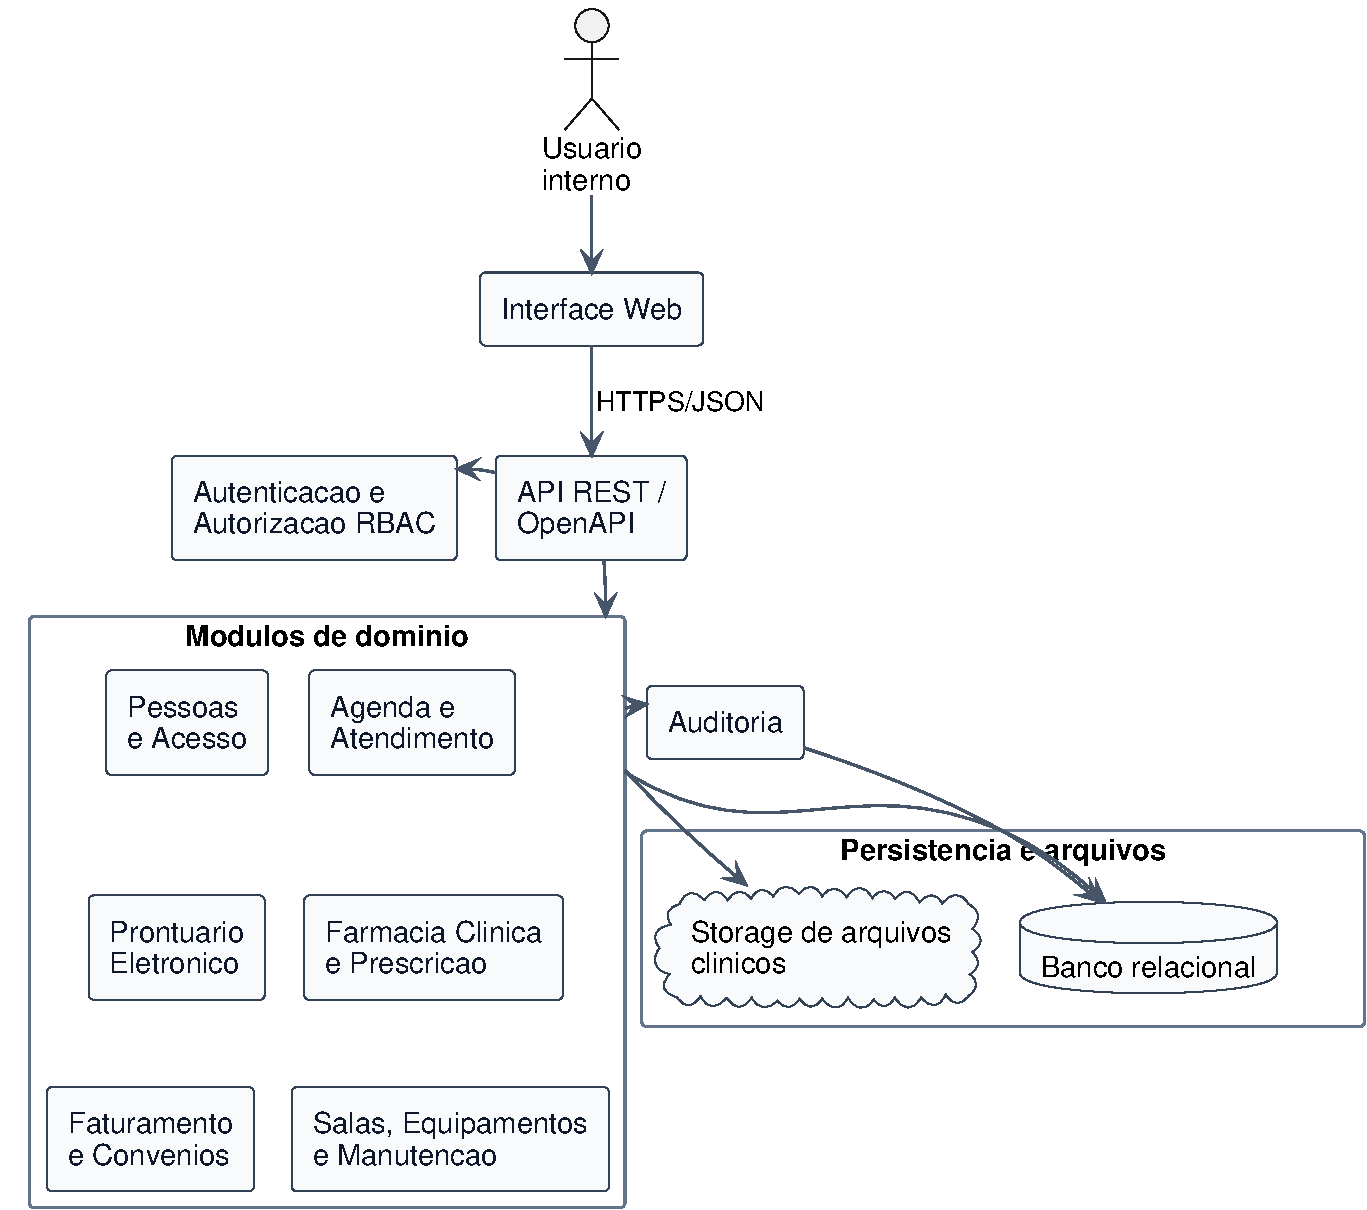
\includegraphics[width=\textwidth,height=0.50\textheight,keepaspectratio]{Imagens/arquitetura/M-V2-01-componentes-logicos}
\caption{Modelo M-V2-01 -- Componentes lógicos do Sistema de Gestão de Clínica.}
\label{fig:m-v2-01-componentes-logicos}
\end{figure}



%% ─────────────────────────────────────────────
\section{Visão de Processos}
 
A visão de processos descreve o comportamento dinâmico e de execução do SGC, tratando
os concerns de desempenho (C2), integridade transacional (C4), rastreabilidade (C5) e
interoperabilidade entre módulos (C8). Ela responde à pergunta: \textit{quais processos
existem em execução e como se comunicam?}
 
\subsection{Modelo de Execução — Arquitetura Cliente/Servidor}
 
O SGC opera segundo uma arquitetura \textbf{Cliente/Servidor} com três processos
principais em execução:
 
\begin{itemize}
    \item \textbf{Processo do Cliente (Navegador/React):} executa no dispositivo do
    usuário e é responsável pela renderização da interface e pelo envio de requisições.
 
    \item \textbf{Processo da API (FastAPI):} executa em contêiner na nuvem e concentra
    toda a lógica de negócio, autenticação, autorização e orquestração dos módulos de
    domínio.
 
    \item \textbf{Processo do Banco de Dados (PostgreSQL/Supabase):} executa como serviço
    gerenciado e é o único responsável pela persistência e atomicidade das transações.
\end{itemize}
 
A comunicação entre o Cliente e a API é \textbf{síncrona}, realizada via
\texttt{HTTPS/REST} com contrato \texttt{JSON}. A comunicação entre a API e o banco é
\textbf{transacional}, utilizando \texttt{SQL} com suporte a transações ACID — garantindo
que operações críticas como agendamento e dispensação sejam atômicas e não gerem estados
inconsistentes em caso de falha parcial.
 
\subsection{Modelo M-V3-01 — Fluxo de Processos}
 
A \autoref{fig:m-v3-01-processos} apresenta o diagrama de componentes da visão de
processos, evidenciando os três processos em execução e os protocolos de comunicação
entre eles.
 
\begin{figure}[htbp]
\centering
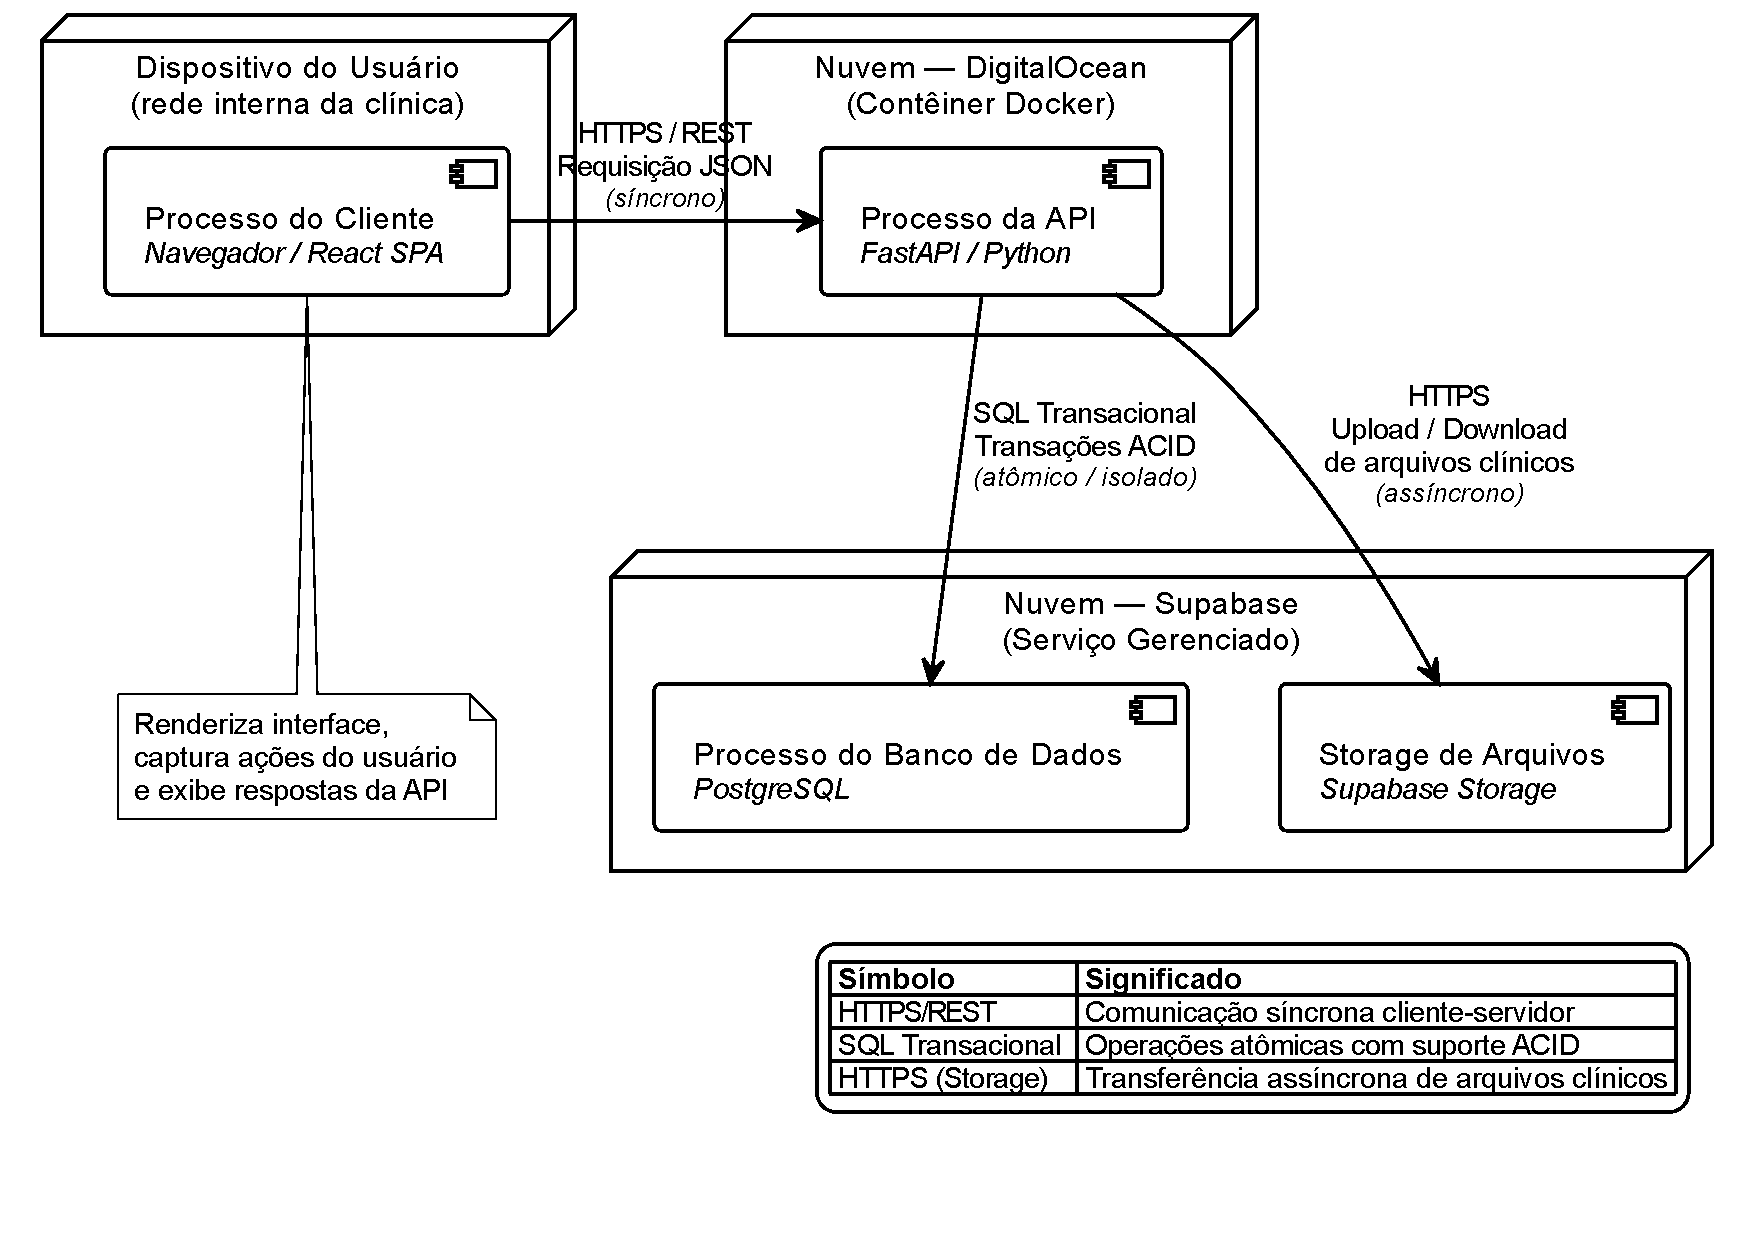
\includegraphics[width=0.85\textwidth,keepaspectratio]{Imagens/arquitetura/M-V3-01-processos.pdf}
\caption{Modelo M-V3-01 — Fluxo de processos e comunicação entre camadas de execução.}
\label{fig:m-v3-01-processos}
\end{figure}
 
\subsection{Controle de Concorrência}
 
Uma consequência direta da arquitetura de processos é o tratamento de concorrência. Quando
dois usuários tentam agendar o mesmo slot horário simultaneamente, a sequência abaixo
garante a integridade dos dados:
 
\begin{enumerate}
    \item Ambos os processos clientes enviam requisições \texttt{POST /consultas} à API
    de forma concorrente.
    \item A API encaminha as duas operações ao banco, que as executa dentro de
    transações isoladas (\textit{serializable isolation}).
    \item O banco concede o bloqueio à primeira transação a chegar; a segunda recebe
    uma exceção de conflito.
    \item A API captura o conflito e retorna \texttt{HTTP 409 Conflict} ao segundo
    cliente, que exibe a mensagem de horário indisponível.
\end{enumerate}
 
Esse mecanismo satisfaz diretamente o concern C4 (integridade transacional) e está
alinhado à decisão arquitetural DA06.
 









%% ─────────────────────────────────────────────
\section{Visão de Desenvolvimento}

A visão de desenvolvimento organiza o sistema em camadas lógicas de responsabilidade, facilitando a compreensão da estrutura de código e suportando os concerns de modularidade (C7), interoperabilidade (C8) e testabilidade (C11).

\subsection{Modelo M-V4-01 -- Camadas}

O modelo M-V4-01 apresenta a organização em camadas do SGC, seguindo o padrão \textit{Layered Architecture}. Cada camada possui responsabilidades bem delimitadas e se comunica somente com a camada adjacente, exceto a camada de Domínio que acessa a Infraestrutura compartilhada para persistência.

\begin{figure}[htbp]
\centering
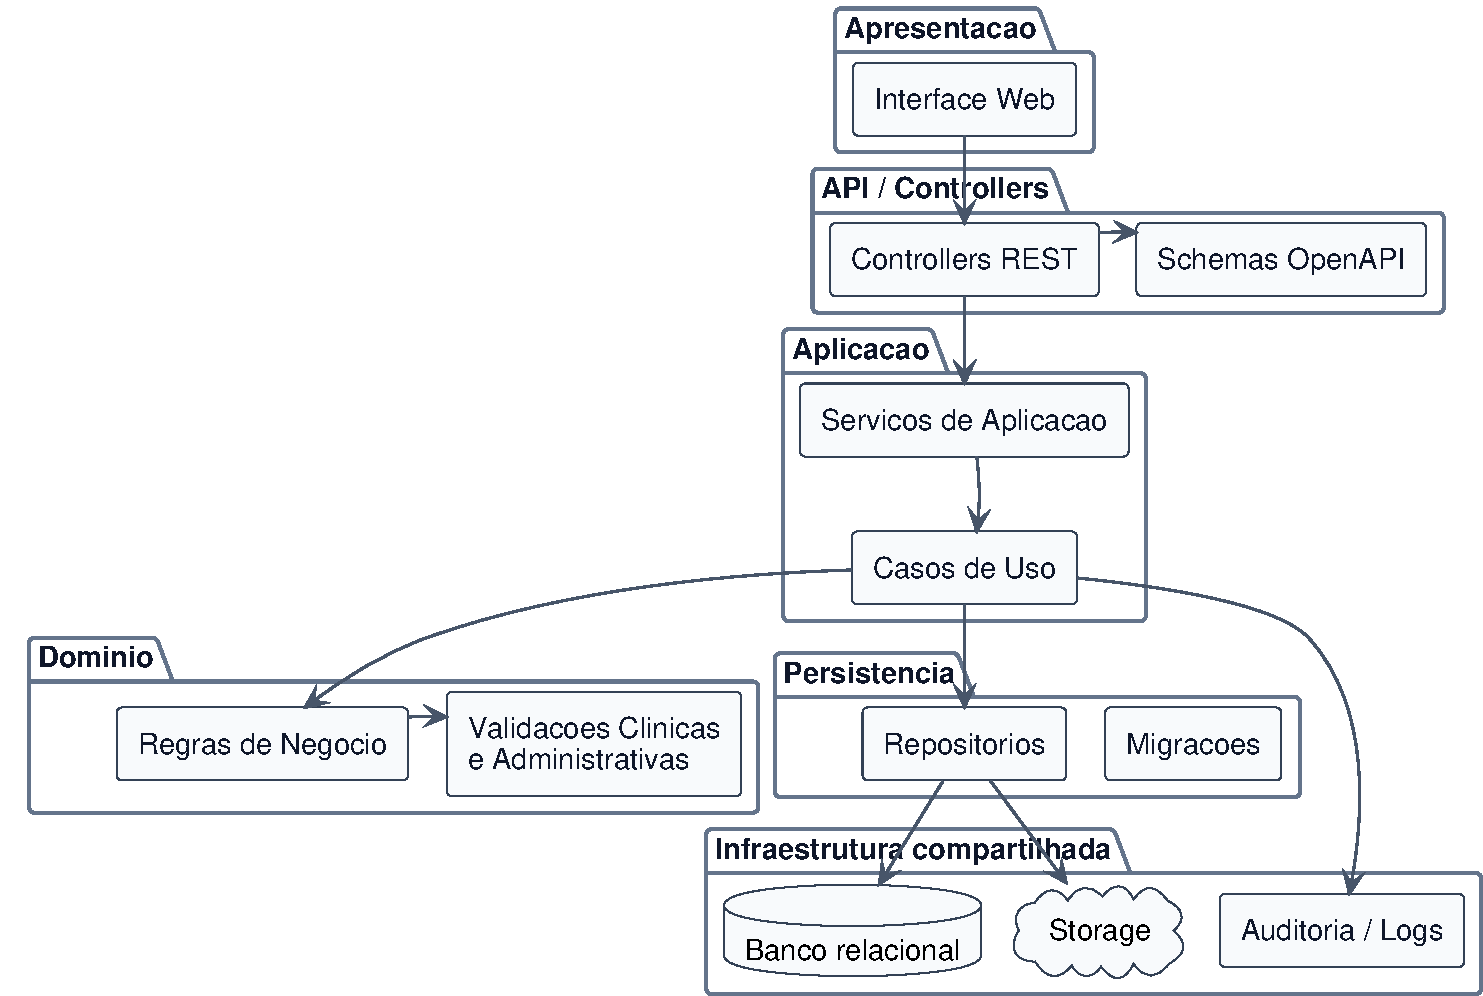
\includegraphics[width=1.0\textwidth,height=0.80\textheight,keepaspectratio]{Imagens/arquitetura/M-V4-01-camadas}
\caption{Modelo M-V4-01 -- Camadas lógicas da aplicação.}
\label{fig:m-v4-01-camadas}
\end{figure}

%% ─────────────────────────────────────────────
\section{Visão Física ou de Implantação}

A visão de implantação descreve a distribuição dos artefatos de software nos nós de execução, endereçando os concerns de disponibilidade (C3), persistência (C10) e operação (C12).

\subsection{Modelo M-V5-01 -- Implantação}

O modelo M-V5-01 mapeia os contêineres de execução e serviços de infraestrutura utilizados pelo SGC. A solução adota plataforma em nuvem com ambientes separados de produção e homologação, pipeline de CI/CD automatizado e serviços gerenciados de banco de dados e armazenamento via Supabase.

\begin{figure}[H]
\centering
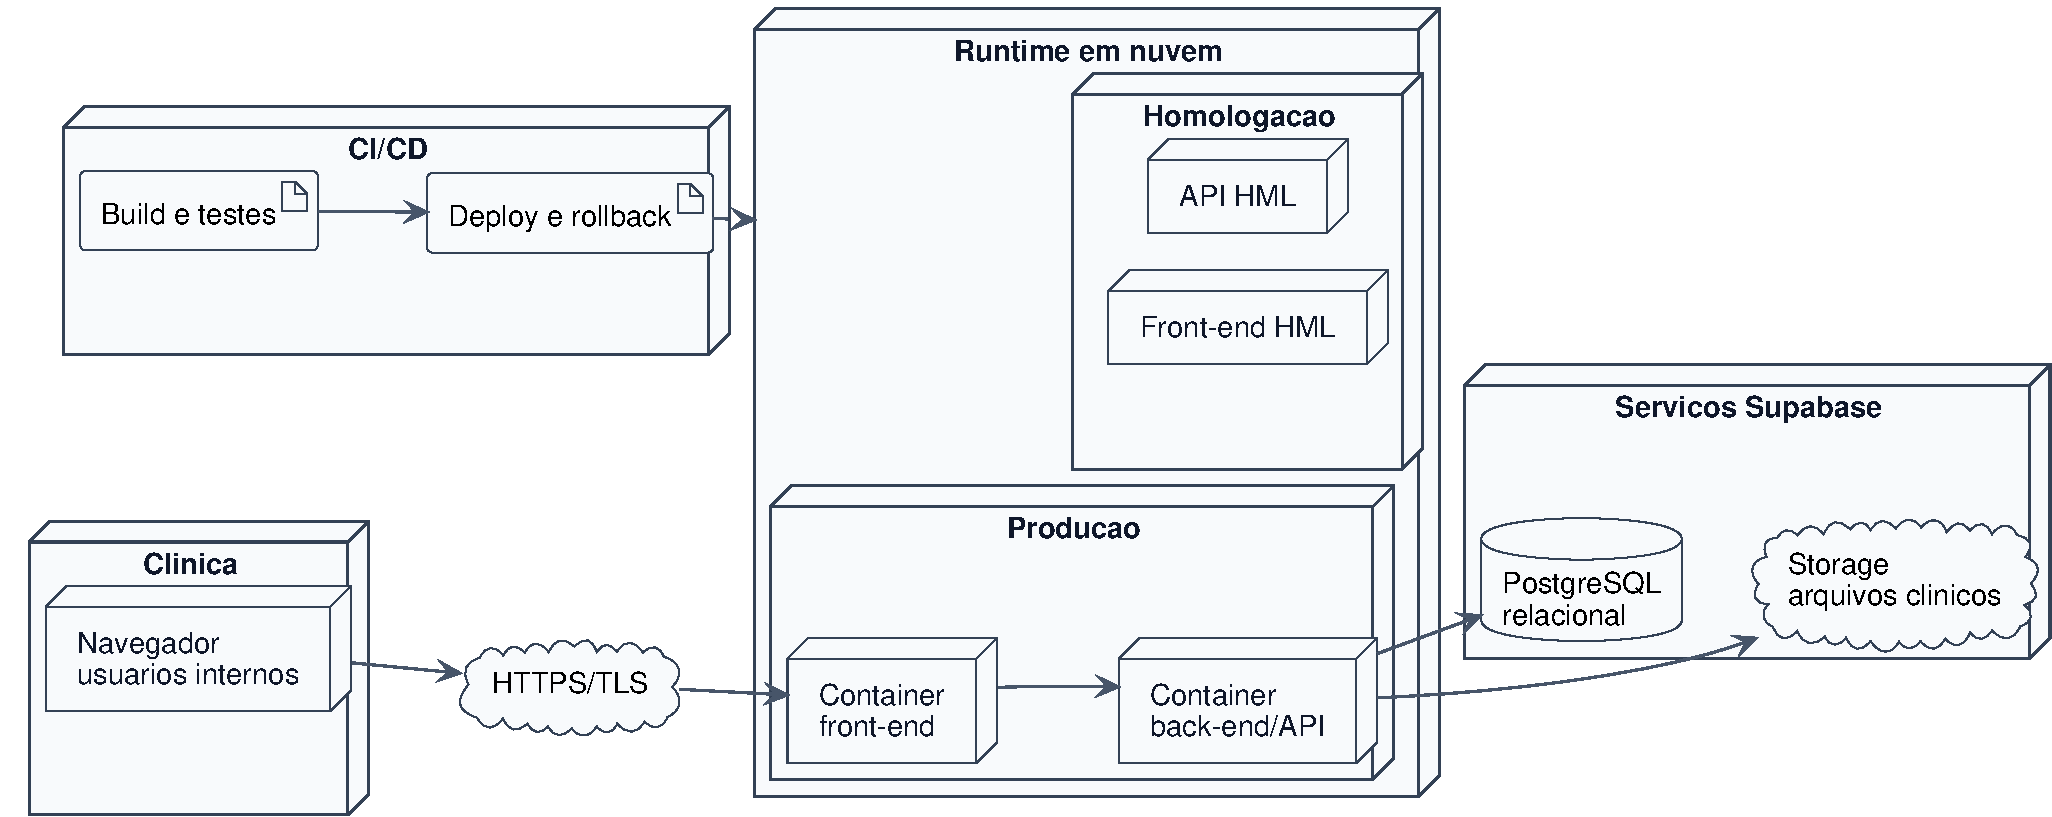
\includegraphics[width=0.82\textwidth,height=0.28\textheight,keepaspectratio]{Imagens/arquitetura/M-V5-01-implantacao}
\caption{Modelo M-V5-01 -- Implantação do Sistema de Gestão de Clínica.}
\label{fig:m-v5-01-implantacao}
\end{figure}
\vspace{-0.8em}

%% ─────────────────────────────────────────────
\section{Visão de Segurança e Conformidade}

A visão de segurança aborda os mecanismos de proteção dos dados e controle de acesso do SGC, endereçando os concerns de segurança (C1), auditoria (C5) e conformidade com LGPD (C6). O controle de acesso é implementado por meio de RBAC (\textit{Role-Based Access Control}), com papéis mapeados às funcionalidades do sistema.

A \autoref{tab:rbac-resumido} apresenta a matriz RBAC resumida com os principais papéis e permissões.

\begin{table}[htbp]
\caption{Matriz RBAC resumida.}
\label{tab:rbac-resumido}
\centering
\small
\begin{tabular}{|l|c|c|c|c|c|}
\hline
\textbf{Funcionalidade} & \textbf{Admin} & \textbf{Médico} & \textbf{Recep.} & \textbf{Farm.} & \textbf{TI} \\
\hline
Cadastro de pacientes      & \checkmark & -- & \checkmark & -- & -- \\
Agendamento de consultas   & \checkmark & \checkmark & \checkmark & -- & -- \\
Prontuário eletrônico      & \checkmark & \checkmark & -- & -- & -- \\
Prescrição médica          & \checkmark & \checkmark & -- & -- & -- \\
Dispensação de medicamentos & \checkmark & -- & -- & \checkmark & -- \\
Gestão de estoque          & \checkmark & -- & -- & \checkmark & -- \\
Faturamento e convênios    & \checkmark & -- & \checkmark & -- & -- \\
Administração de usuários  & \checkmark & -- & -- & -- & \checkmark \\
Auditoria e logs           & \checkmark & -- & -- & -- & \checkmark \\
\hline
\end{tabular}
\end{table}

\needspace{6\baselineskip}
\subsection{Modelo M-V6-01 -- Controles de Segurança}

O modelo M-V6-01 detalha os componentes de segurança do SGC e suas interações. O ponto de controle central é o \textit{back-end/API}, que intercepta todas as requisições e as submete ao Serviço de Autenticação e ao Serviço de Autorização RBAC antes de processar qualquer operação. Dados sensíveis de pacientes são armazenados em \textit{storage} protegido com criptografia em repouso, em conformidade com a LGPD.

\begin{figure}[htbp]
\centering
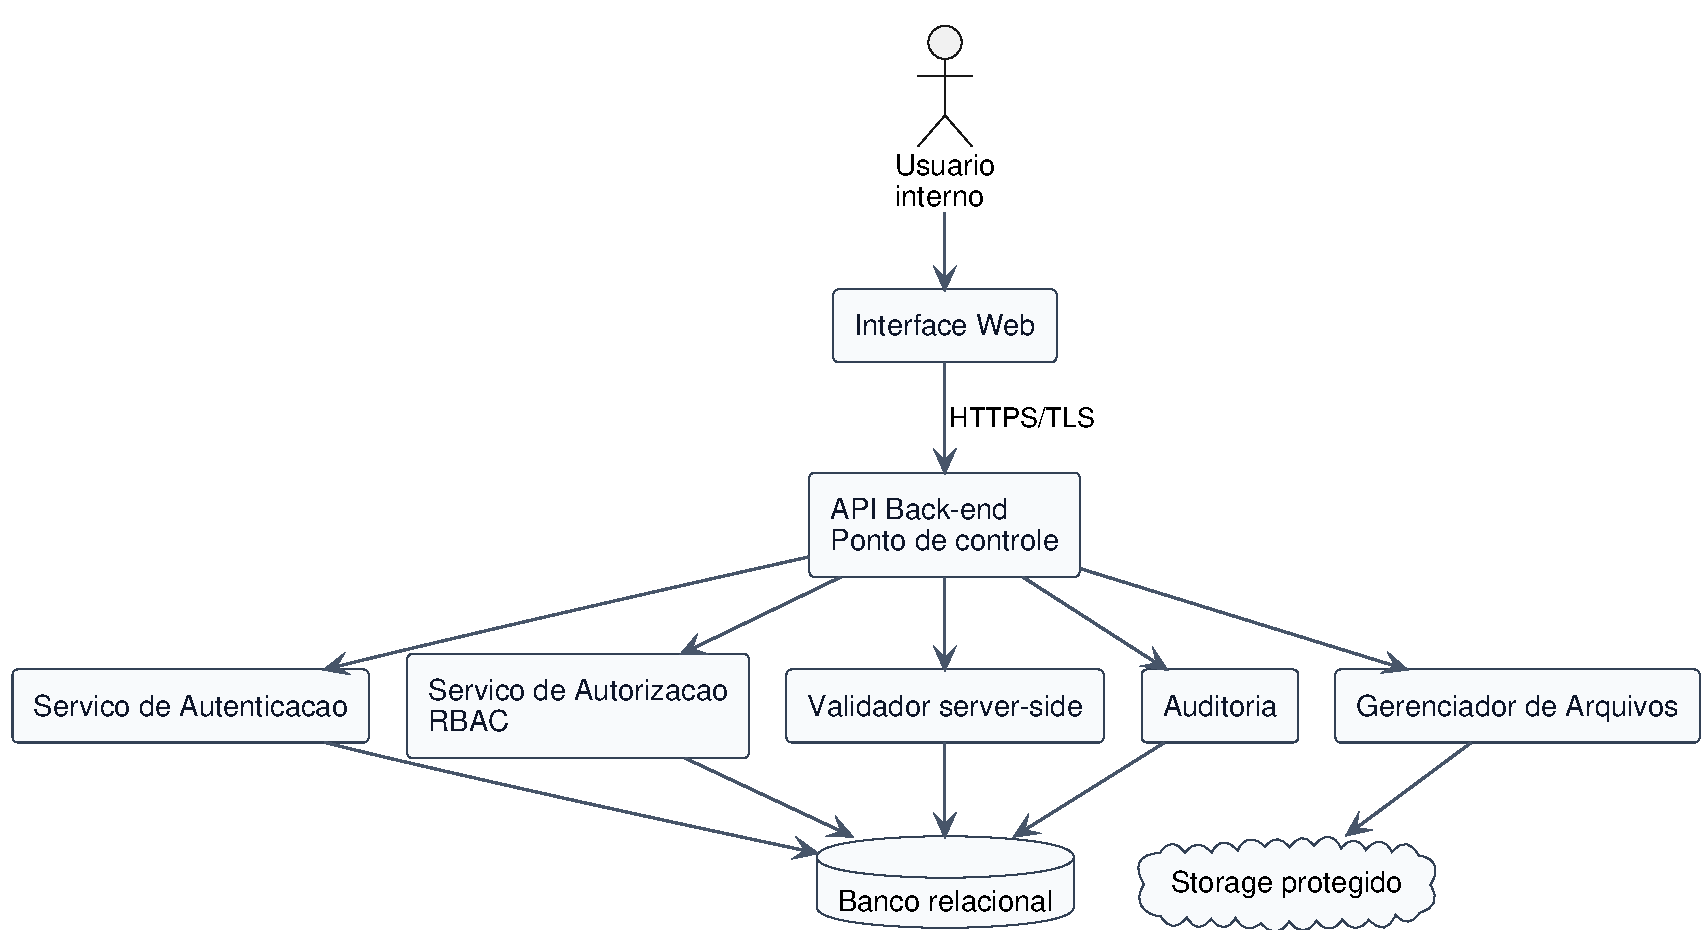
\includegraphics[width=0.85\textwidth,height=0.55\textheight,keepaspectratio]{Imagens/arquitetura/M-V6-01-seguranca}
\caption{Modelo M-V6-01 -- Controles de segurança e conformidade.}
\label{fig:m-v6-01-seguranca}
\end{figure}

%% ─────────────────────────────────────────────
\section{Correspondências e Regras de Consistência}

Seguindo a ISO 42010, as correspondências (\textit{correspondences}) explicitam as relações entre elementos de diferentes views, garantindo consistência interna da descrição arquitetural.

A \autoref{tab:correspondence-rules} define as regras de correspondência estabelecidas para o SGC.

\begin{table}[htbp]
\caption{Regras de correspondência arquitetural.}
\label{tab:correspondence-rules}
\centering
\small
\begin{tabularx}{\textwidth}{|l|X|}
\hline
\textbf{Regra} & \textbf{Definição} \\
\hline
CR-01 & Todo componente presente em V2 (Lógica) deve ter pelo menos um participante correspondente nos diagramas de sequência de V1 ou V3. \\
CR-02 & Todo módulo de domínio em V2 deve ter um contêiner correspondente no diagrama de implantação V5. \\
CR-03 & Todo fluxo com dados sensíveis de pacientes em V1 ou V3 deve passar pelo autorizacaoService documentado em V6. \\
CR-04 & Toda operação de escrita nos diagramas V1 e V3 deve incluir chamada ao auditoriaService. \\
\hline
\end{tabularx}
\end{table}

A \autoref{tab:correspondencias} instancia as correspondências identificadas entre os elementos das views.

\begin{table}[htbp]
\caption{Correspondências arquiteturais.}
\label{tab:correspondencias}
\centering
\small
\begin{tabularx}{\textwidth}{|l|l|l|X|}
\hline
\textbf{ID} & \textbf{Elemento em} & \textbf{Corresponde em} & \textbf{Elemento correspondente} \\
\hline
CO-01 & ConsultaController (V1) & V2 & Módulo Agenda e Atendimento \\
CO-02 & DispensacaoController (V3) & V2 & Módulo Farmácia Clínica e Prescrição \\
CO-03 & autorizacaoService (V1, V3) & V6 & Serviço de Autorização RBAC \\
CO-04 & auditoriaService (V1, V3) & V6 & Auditoria \\
CO-05 & consultaRepository (V1) & V5 & Contêiner back-end/API → Supabase PostgreSQL \\
CO-06 & dispensacaoRepository (V3) & V5 & Contêiner back-end/API → Supabase PostgreSQL \\
\hline
\end{tabularx}
\end{table}

\subsection{Conformidade com o ArchCaMo}

A \autoref{tab:conformidade-archcamo} avalia o grau de conformidade desta descrição arquitetural com os critérios do ArchCaMo.

\begin{table}[htbp]
\caption{Conformidade da descrição arquitetural com o ArchCaMo.}
\label{tab:conformidade-archcamo}
\centering
\small
\begin{tabularx}{\textwidth}{|l|X|c|}
\hline
\textbf{Critério} & \textbf{Evidência neste documento} & \textbf{Status} \\
\hline
Concerns identificados       & Tabela~\ref{tab:concerns-arquitetura}: 12 concerns explícitos & \checkmark \\
Stakeholders documentados    & Tabela~\ref{tab:stakeholders-arquitetura}: 11 stakeholders & \checkmark \\
Viewpoints definidos         & Tabela~\ref{tab:viewpoints-visoes}: 6 viewpoints & \checkmark \\
Views com modelos            & M-V1-01 a M-V6-01 & \checkmark \\
Correspondências explícitas  & Tabelas~\ref{tab:correspondence-rules} e~\ref{tab:correspondencias}: 4 regras e 6 correspondências & \checkmark \\
Decisões arquiteturais       & Tabela~\ref{tab:decisoes-arquiteturais}: 8 decisões & \checkmark \\
Rastreabilidade              & Tabela~\ref{tab:rastreabilidade}: concerns × views × modelos × decisões & \checkmark \\
Model kinds declarados       & Tabela~\ref{tab:viewpoints-visoes}: UML Sequence, Component e Deployment & \checkmark \\
Rationale documentado        & Seção~\ref{sec:rationale}: rationale de 5 decisões principais & \checkmark \\
Consistência verificada      & CR-01 a CR-04 verificadas pelas correspondências CO-01 a CO-06 & \checkmark \\
\hline
\end{tabularx}
\end{table}

%% ─────────────────────────────────────────────
\section{Decisões Arquiteturais e Rationale}

As decisões arquiteturais registram as escolhas de design significativas que moldaram a estrutura do SGC, juntamente com a justificativa (\textit{rationale}) e as alternativas consideradas. A \autoref{tab:decisoes-arquiteturais} sintetiza as principais decisões.

\begin{table}[htbp]
\caption{Decisões arquiteturais resumidas.}
\label{tab:decisoes-arquiteturais}
\centering
\small
\begin{tabularx}{\textwidth}{|l|X|l|}
\hline
\textbf{ID} & \textbf{Decisão} & \textbf{Concerns} \\
\hline
DA01 & Adotar arquitetura em camadas (Apresentação, API, Aplicação, Domínio, Persistência) & C7, C8, C11 \\
DA02 & Expor API REST com contrato OpenAPI/Swagger & C8, C9 \\
DA03 & Implementar controle de acesso via RBAC com papéis pré-definidos & C1, C6 \\
DA04 & Adotar persistência relacional gerenciada e storage separado para arquivos clínicos (concretizada via Supabase) & C3, C10, C12 \\
DA05 & Adotar interface web SPA responsiva para fluxos operacionais (concretizada via React) & C9, C2 \\
DA06 & Operações críticas encapsuladas em transações atômicas no banco & C4 \\
DA07 & Serviço de auditoria centralizado chamado por todos os controllers & C5, C6 \\
DA08 & Pipeline CI/CD automatizado com ambientes de produção e homologação & C12, C3 \\
\hline
\end{tabularx}
\end{table}

\subsection{Rationale das Decisões Principais}
\label{sec:rationale}

\textbf{DA01 -- Arquitetura em Camadas:} A separação em camadas distintas (Apresentação, API, Aplicação, Domínio e Persistência) promove alta coesão e baixo acoplamento, facilitando testes unitários e a evolução independente de cada camada. A alternativa de microserviços foi descartada pela complexidade operacional incompatível com o tamanho da equipe e o prazo do projeto.

\textbf{DA03 -- RBAC:} O controle de acesso baseado em papéis permite gerenciar permissões de forma centralizada e auditável, sem necessidade de lógica de autorização distribuída nos módulos. Essa abordagem atende diretamente ao C1 e ao C6 (LGPD), evitando exposição indevida de dados sensíveis de pacientes.

\textbf{DA04 -- Persistência Relacional Gerenciada:} Adotar um banco relacional gerenciado (PostgreSQL via Supabase) com storage separado para arquivos clínicos reduz a carga operacional de configuração de infraestrutura de dados, permitindo que a equipe foque nas regras de negócio. O suporte a transações ACID atende C4; o storage separado satisfaz C10 e C6 (arquivos de pacientes cifrados em repouso).

\textbf{DA06 -- Transações Atômicas:} Operações como agendamento e dispensação envolvem múltiplas escritas que devem ser indivisíveis. O uso de transações de banco de dados garante que, em caso de falha parcial, nenhum estado inconsistente seja persistido, satisfazendo C4.

\textbf{DA07 -- Auditoria Centralizada:}\ Centralizar o registro de auditoria em um serviço dedicado (\texttt{auditoriaService}) garante que nenhuma operação crítica escape do rastreamento, independentemente do módulo que a dispara. Isso simplifica a conformidade com LGPD e facilita investigações.

%% ─────────────────────────────────────────────
\section{Rastreabilidade entre Concerns, Views, Modelos e Decisões}

A \autoref{tab:rastreabilidade} apresenta a matriz de rastreabilidade que relaciona cada concern arquitetural às views, modelos e decisões que o endereçam, demonstrando a completude da descrição arquitetural.

\begin{table}[H]
\caption{Rastreabilidade entre concerns, stakeholders, views, modelos e decisões.}
\label{tab:rastreabilidade}
\centering
\small
\begin{tabularx}{\textwidth}{|l|X|l|l|l|}
\hline
\textbf{Concern} & \textbf{Stakeholders} & \textbf{Views} & \textbf{Modelos} & \textbf{Decisões} \\
\hline
C1  & S3, S9               & V1, V6     & M-V1-01, M-V6-01                    & DA03, DA07 \\
C2  & S4, S5, S10          & V3         & M-V3-01                             & DA02, DA05 \\
C3  & S8                   & V5         & M-V5-01                             & DA04, DA08 \\
C4  & S2, S4, S5, S6, S7   & V1, V3     & M-V1-01, M-V3-01                    & DA06       \\
C5  & S3, S6, S9, S11      & V1, V3, V6 & M-V1-01, M-V3-01, M-V6-01          & DA07       \\
C6  & S3, S9               & V6         & M-V6-01                             & DA03, DA07 \\
C7  & S1, S2               & V2, V4     & M-V2-01, M-V4-01                    & DA01       \\
C8  & S1, S2               & V2, V3, V4 & M-V2-01, M-V3-01, M-V4-01          & DA02       \\
C9  & S4, S5, S7, S10, S11 & V2         & M-V2-01                             & DA05, DA02 \\
C10 & S6, S7, S8           & V2, V5     & M-V2-01, M-V5-01                    & DA04       \\
C11 & S1, S2               & V4         & M-V4-01                             & DA01       \\
C12 & S8, S11              & V5         & M-V5-01                             & DA04, DA08 \\
\hline
\end{tabularx}
\end{table}
\chapter{Status dos Casos de Uso}

Este capítulo apresenta o estado atual de implementação dos casos de uso definidos na Entrega~2 do projeto. O desenvolvimento do SGC adota uma abordagem incremental, priorizando os fluxos de maior impacto operacional. O protótipo funcional da interface foi desenvolvido com a stack definida na arquitetura --- React no front-end, com integração prevista à API FastAPI e ao banco de dados PostgreSQL via Supabase.

\section{Visão Geral do Estado de Implementação}

A \autoref{tab:status-ucs} consolida a situação de cada caso de uso, classificando-o em uma das três categorias: \textbf{Funcional} (tela implementada, navegação ativa e dados de demonstração integrados), \textbf{Parcial} (funcionalidade presente como subcomponente de outro módulo) ou \textbf{Planejado} (escopo definido, implementação não iniciada).

\renewcommand{\arraystretch}{1.3}
\begin{table}[H]
\centering
\small
\begin{tabularx}{\textwidth}{|p{1.2cm}|p{5.2cm}|p{2.8cm}|X|}
\hline
\textbf{ID} & \textbf{Caso de Uso} & \textbf{Status} & \textbf{Observação} \\ \hline
UC01 & Gerenciar Cadastro de Pacientes   & Funcional & Tabela de pacientes com busca por nome/CPF, indicadores de status, formulário de cadastro e edição, e ação de inativação. \\ \hline
UC02 & Gerenciar Agenda de Consultas     & Funcional & Calendário semanal com filtro por profissional, codificação visual por status e botão de novo agendamento. \\ \hline
UC03 & Configurar Grade de Horários      & Planejado           & Definido no escopo; implementação prevista para fase seguinte. \\ \hline
UC04 & Realizar Atendimento Clínico      & Funcional & Prontuário eletrônico com sinais vitais, histórico de atendimentos por CID, anamnese estruturada (queixa principal, HDA, conduta) e abas de receita e documentos. \\ \hline
UC05 & Emitir Prescrição Médica          & Parcial             & Aba ``Receita'' presente no módulo de Prontuário com lista de medicamentos e geração de PDF. \\ \hline
UC06 & Dispensar Medicamentos            & Planejado           & Definido no escopo; fluxo de dispensação previsto para integração com o módulo de farmácia. \\ \hline
UC07 & Gerenciar Estoque Farmacêutico    & Funcional & Inventário com código, lote, quantidade, mínimo, validade e alertas automáticos de ruptura. \\ \hline
UC08 & Faturar Atendimento               & Planejado           & Definido no escopo; módulo financeiro previsto para fase seguinte. \\ \hline
UC09 & Administrar Usuários e Permissões & Parcial             & Autenticação com seleção de perfil RBAC implementada na tela de login; gestão administrativa não implementada. \\ \hline
UC10 & Gerenciar Salas e Equipamentos    & Planejado           & Definido no escopo; módulo de infraestrutura previsto para fase seguinte. \\ \hline
\end{tabularx}
\caption{Status de implementação dos casos de uso do SGC}
\label{tab:status-ucs}
\end{table}

\section{Casos de Uso Funcionais}

As seções a seguir apresentam as telas implementadas para os três casos de uso destacados neste incremento, com descrição das funcionalidades disponíveis em cada módulo.

%%────────────────────────────────────────────────
\subsection{UC01 --- Gerenciar Cadastro de Pacientes}

O módulo de Cadastro de Pacientes exibe três indicadores no topo: total cadastrado, ativos e inativos. A tabela lista cada paciente com nome, CPF, data de nascimento, telefone, convênio e status colorido (\textbf{Ativo} em verde, \textbf{Inativo} em cinza), com ações de \textbf{edição} e \textbf{inativação}. O botão ``Novo paciente'' abre formulário inline com validação de CPF duplicado.

\begin{figure}[htbp]
\centering
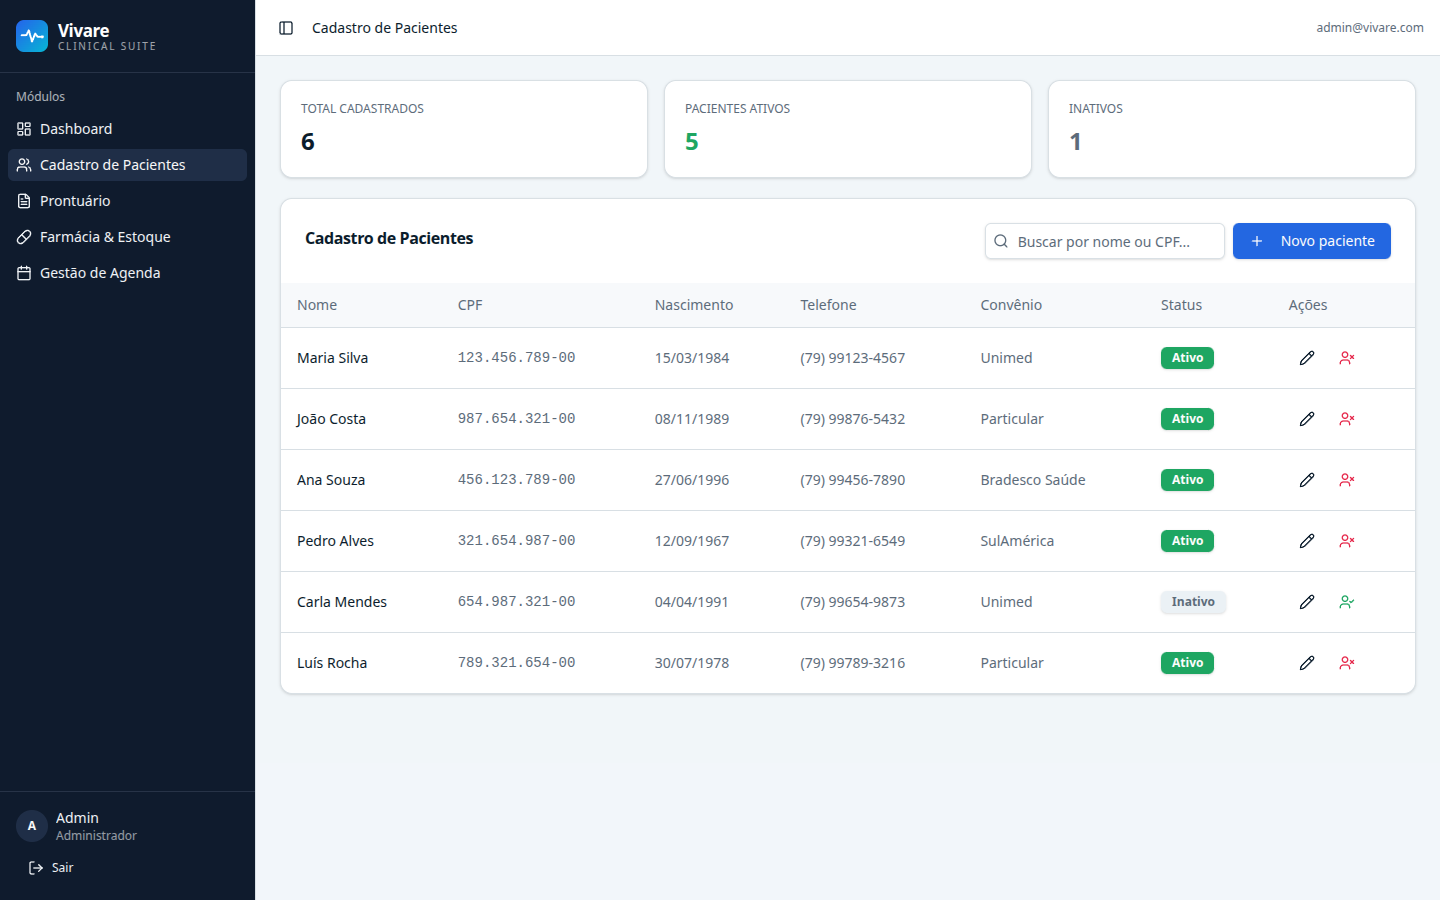
\includegraphics[width=\textwidth,height=0.37\textheight,keepaspectratio]{Imagens/cap6-tela-pacientes.png}
\caption{Tela do módulo Cadastro de Pacientes --- UC01}
\label{fig:cap6-pacientes}
\end{figure}

%%────────────────────────────────────────────────
\subsection{UC02 --- Gerenciar Agenda de Consultas}

O módulo de Gestão de Agenda implementa visão semanal com navegação entre semanas e filtro por profissional. Cada compromisso exibe nome do paciente, médico responsável e código de cor por status: \textbf{confirmado} (azul), \textbf{em atendimento} (verde), \textbf{aguardando} (cinza) e \textbf{conflito} (vermelho). O botão ``Novo agendamento'' está disponível na barra de controles.

\begin{figure}[htbp]
\centering
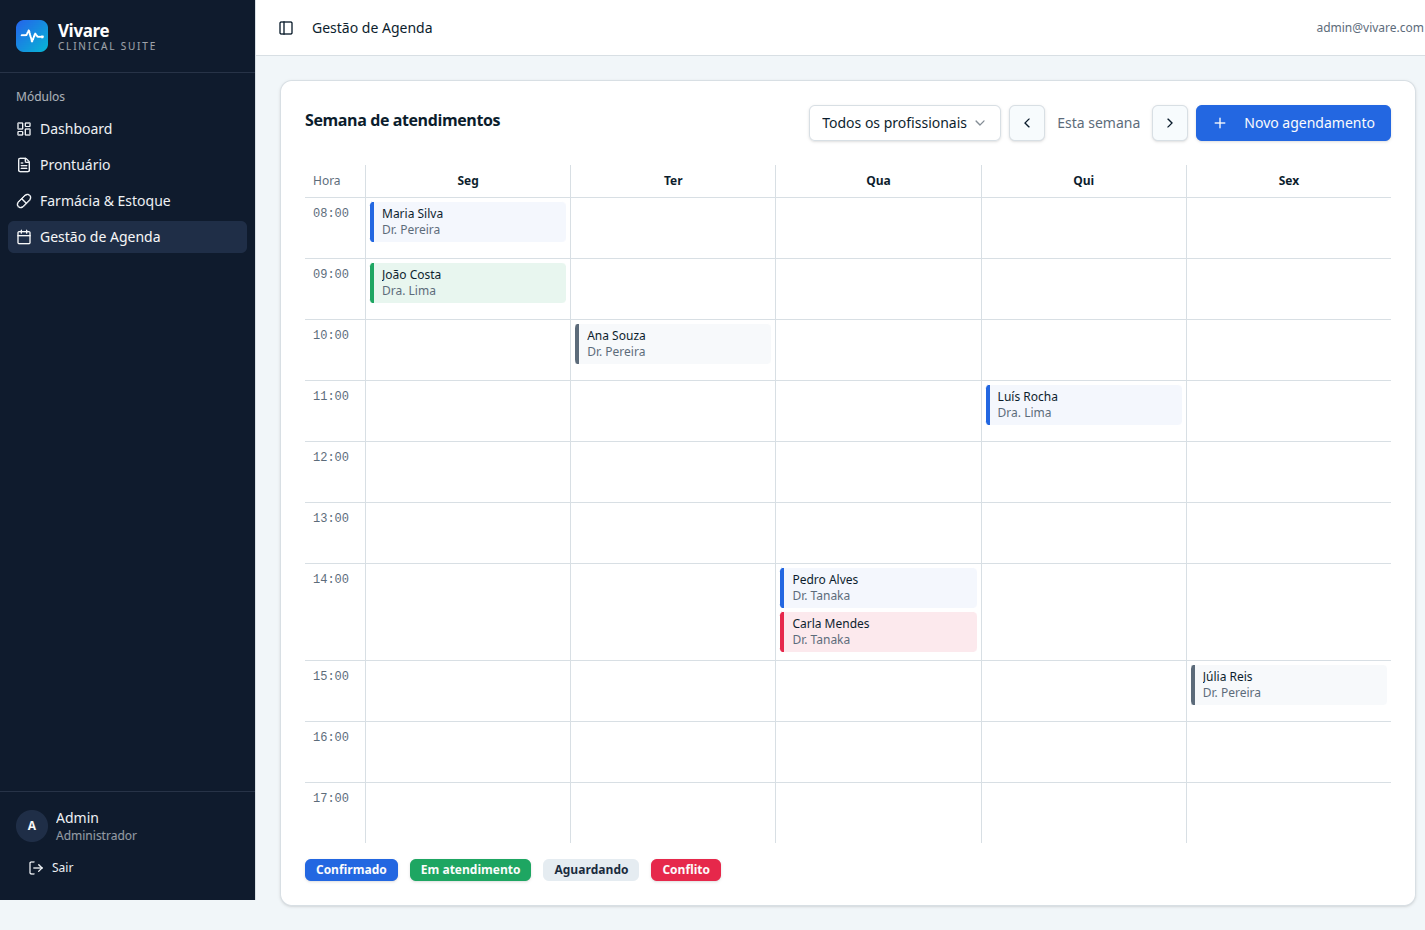
\includegraphics[width=\textwidth,height=0.37\textheight,keepaspectratio]{Imagens/cap6-tela-agenda.png}
\caption{Tela do módulo Gestão de Agenda --- UC02}
\label{fig:cap6-agenda}
\end{figure}

%%────────────────────────────────────────────────
\subsection{UC04 --- Realizar Atendimento Clínico}

O módulo de Prontuário Eletrônico apresenta busca de pacientes em tempo real. Ao selecionar um paciente, o painel exibe: dados cadastrais com tipo sanguíneo e alergias em destaque, seis sinais vitais (PA, FC, temperatura, SpO\textsubscript{2}, peso e IMC) e histórico de atendimentos anteriores com data, CID, diagnóstico, médico e tipo de visita. A evolução clínica é registrada em campos estruturados de \textbf{queixa principal}, \textbf{HDA} e \textbf{conduta}, com abas de \textbf{Receita} e \textbf{Documentos}.

\begin{figure}[htbp]
\centering
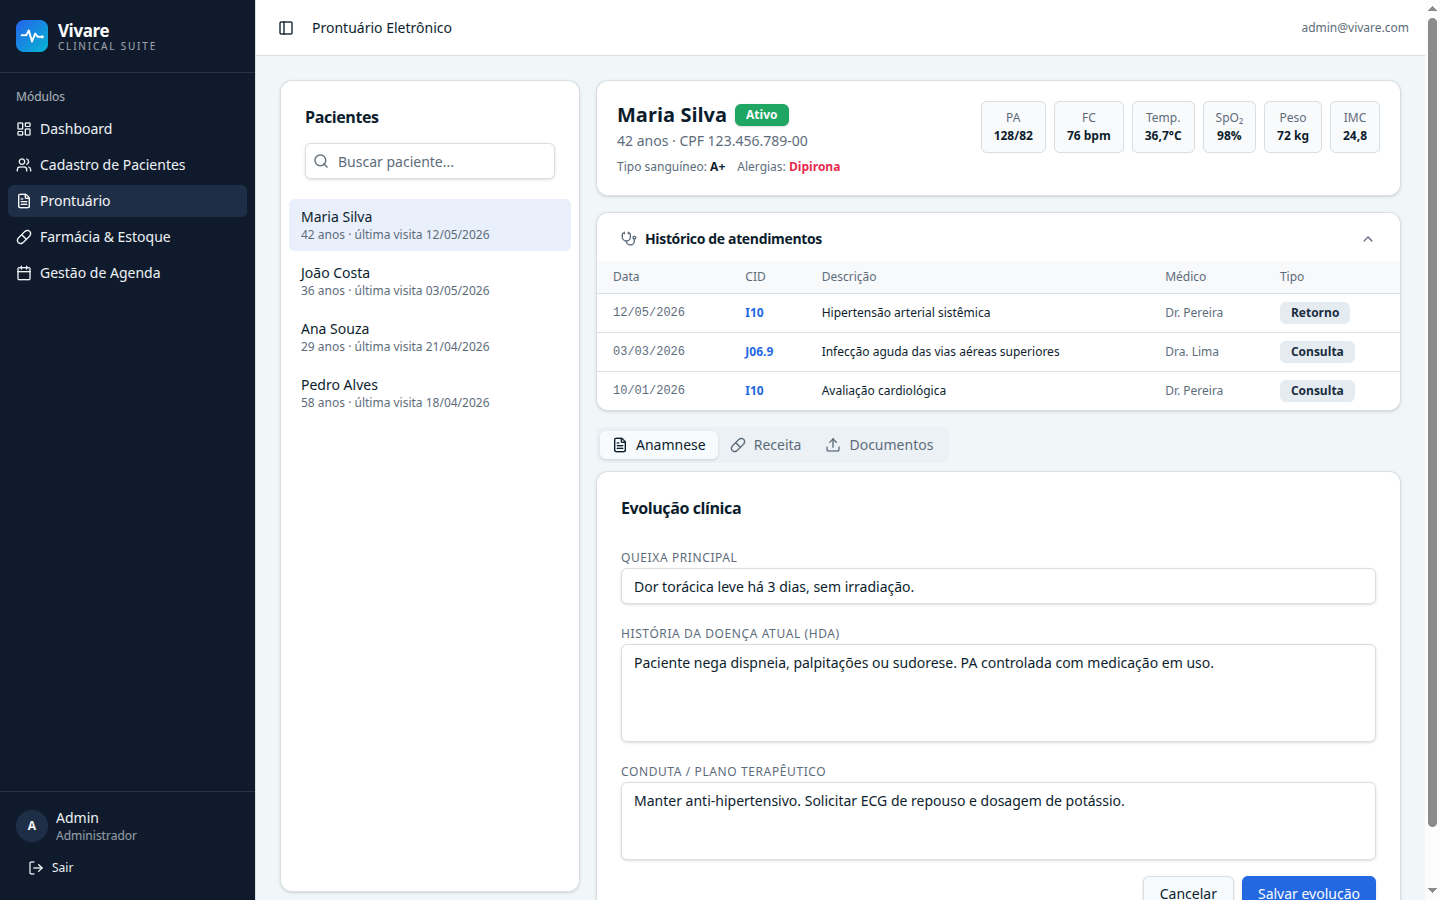
\includegraphics[width=\textwidth,height=0.37\textheight,keepaspectratio]{Imagens/cap6-tela-prontuario.png}
\caption{Tela do módulo Prontuário Eletrônico --- UC04}
\label{fig:cap6-prontuario}
\end{figure}

\section{Considerações sobre os Próximos Incrementos}

Os casos de uso classificados como \textbf{Planejado} (UC03, UC06, UC08 e UC10) têm seus fluxos completamente especificados na Entrega~2 e suas entidades mapeadas no modelo objeto-relacional deste documento. A prioridade para o próximo incremento é UC06 (Dispensar Medicamentos), que complementa diretamente o módulo de farmácia já disponível, e UC08 (Faturar Atendimento), cujos dados de entrada já são produzidos pelos módulos de agenda e prontuário implementados.

\phantompart
%\bibliography{Bibliografia}

%%%%%%%%%%%%%%%%%%%%%%%%%%%%%%%%%%%%%%%%%%%%%%%%%%%%%%%%%%%%%%%%%%%%%%%%%%
% ELEMENTOS PÓS-TEXTUAIS
%%%%%%%%%%%%%%%%%%%%%%%%%%%%%%%%%%%%%%%%%%%%%%%%%%%%%%%%%%%%%%%%%%%%%%%%%%

\postextual

\renewcommand{\chapnumfont}{\chaptitlefont}
\renewcommand{\afterchapternum}{}


\end{document}
